\documentclass{my_paper}
\usepackage{subfigure}
\usepackage{ctex}
\usepackage{booktabs}
\usepackage[textwidth=438bp,vmargin=2.5cm]{geometry}%设置页边距
\usepackage{array} %主要是增加列样式选项
\usepackage[dvipsnames]{xcolor}%颜色宏包
\usepackage{graphicx}%图片宏包
\usepackage{amsmath,bm}%公式宏包
\usepackage[T1]{fontenc}
\usepackage{multirow}    
\usepackage{newtxtext, newtxmath}  %两种使用Times New Roman 字体的方法
\newcommand{\subsubsubsection}[1]{\paragraph{#1}\mbox{}\\}
\setcounter{secnumdepth}{4} % how many sectioning levels to assign numbers to
\setcounter{tocdepth}{4} % how many sectioning levels to show in ToC
\linespread{1.5}


\usepackage{listings}
\usepackage{color}
\definecolor{dkgreen}{rgb}{0,0.6,0}
\definecolor{gray}{rgb}{0.5,0.5,0.5}
\definecolor{mauve}{rgb}{0.58,0,0.82}
\lstset{frame=tb,
  language=Matlab,
  aboveskip=3mm,
  belowskip=3mm,
  showstringspaces=false,
  columns=flexible,
  basicstyle={\small\ttfamily},
  numbers=left,%设置行号位置none不显示行号
  %numberstyle=\tiny\courier, %设置行号大小
  numberstyle=\tiny\color{gray},
  keywordstyle=\color{blue},
  commentstyle=\color{dkgreen},
  stringstyle=\color{mauve},
  breaklines=true,
  breakatwhitespace=true,
  escapeinside=``,%逃逸字符(1左面的键),用于显示中文例如在代码中`中文...`
  tabsize=4,
  extendedchars=false %解决代码跨页时,章节标题,页眉等汉字不显示的问题
}

\begin{document}
%----------- 中文摘要 ----------
\newpage

\begin{center}
\lunwenbiaoti

\vspace{2ex}
\zhaiyao
\end{center}

本文针对\textbf{波浪能装置}运动状态和最优参数的计算问题,从装置的受力情况出发,在浮子只做垂荡运动和只做垂荡与纵摇运动两种情况下,分别求解浮子和振子的运动状态。在浮子只做垂荡运动时,分别考虑阻尼系数恒定与变化的两种情况,求解出装置的最大平均输出功率以及对应的最优阻尼系数(比例系数,幂指数);在浮子只做垂荡和纵摇两种运动时,求解出装置的最大平均输出功率及对应的最优阻尼系数。



\textbf{针对问题一},对浮子和振子进行受力分析,并基于牛顿第二定律和\textbf{微分方程}建立浮子与振子的动力学模型,并根据题目信息求得浮子与振子的初值。在求解过程中,使用变量替换,将二阶微分方程组转化为一阶微分方程组,基于\textbf{四五阶龙格-库塔法},针对直线阻尼器的阻尼系数为定值和阻尼系数与浮子和振子的相对速度的绝对值的幂成正比两种情况,求解出浮子与振子在40个波浪周期内时间间隔为0.2$s$的垂荡位移和速度。两种情况下浮子与振子运动状态变化曲线均在短时间震荡后进行较为稳定的周期变换,结果存放在result-1.xlsx和result-2.xlsx文件中。

\textbf{针对问题二},建立\textbf{单目标优化模型}。首先,确定优化目标——平均输出功率最大;其次,当阻尼系数为常量,确定约束条件为阻尼系数的取值界限;当阻尼系数为变量,确定约束条件为比例系数和幂指数的取值界限。然后,基于问题一建立的动力学模型,对时间进行离散化处理。最后,基于\textbf{粒子群算法},求解得到最大平均输出功率及最优阻尼系数(比例系数和幂指数)。当阻尼系数为常量时,最大平均输出功率为246.118$W$,最优阻尼系数为37667.1025$N\cdot s/m$;当阻尼系数为变量时,最大平均输出功率为1216.1029$W$,比例系数和幂指数分别为99643.3182,1。


\textbf{针对问题三},综合考虑浮子做垂荡运动和纵摇运动两种运动前,先考虑浮子只做纵摇运动,对浮子和振子进行受力分析,基于牛顿第二定律,建立该情况下的浮子与振子的动力学模型。然后结合问题一中的模型,考虑浮子做垂荡运动和纵摇运动的耦合关系,建立修正后的浮子和振子的动力学模型。然后,确定初值条件,基于四五阶龙格-库塔法,求解出浮子与振子在40个波浪周期内时间间隔为0.2$s$的垂荡位移与速度和纵摇角位移与角速度。浮子与振子的运动状态均在经历短时间震荡后进行稳定的周期变换,结果保存在result3.xlsx。

\textbf{针对问题四},建立单目标优化模型。首先,确定优化目标——直线阻尼器和旋转阻尼器的平均输出功率之和最大,确定约束条件为直线阻尼器和旋转阻尼器的阻尼系数的取值界限。然后,基于问题三建立的修正的动力学模型,对时间进行离散化处理。最后,基于粒子群算法,求解得到最大平均输出功率为293.624$W$,直线阻尼器和旋转阻尼器的最优阻尼系数分别为56567.4276$N\cdot s/m$,56567.079$N\cdot m \cdot s$。

最后,探究了模型对离散化时间间隔$\Delta t$的灵敏度,分析了模型的优缺点,提出了未来的改进方向。


\begin{guanjianci}
\quad \textbf{波浪能装置} \quad \textbf{微分方程} \quad \textbf{龙格-库塔法} \quad \textbf{单目标优化} \quad \textbf{粒子群算法}
\end{guanjianci}

%----------- 正文 ----------
%----------- 一、问题重述 ----------
\newpage
\section{一、问题重述}
现如今,世界传统能源储量与环保问题的逐渐凸显,为了摆脱传统能源带来的束缚和危害,越来越多的
国家将目光投向新能源领域。
在其中,最受关注的风能和太阳能已经为人类带来了巨大的经济和环保价值,除此之外,波浪能也成为了
学术和工业界一大热点,引领着未来新能源领域的发展方向。

波浪能可由波浪能发电系统转化为电能。目前波浪能发电系统已经有了多种多样的分类,但通常来讲都是由波浪能转化系统(WEC)、波浪能输出系统(PTO)以及多种辅助系统组成。
目前,这样的波浪能发电系统已经在工业界得到应用,但如何设置合理的控制参数,得到更高的转换效率
仍然是一个亟需解决的问题。


在所给附件中,附件1说明了波浪能转换装置在进行垂荡运动下的具体运动情况,附件2为波浪能转换装置
在同时进行垂荡和纵摇运动时的运动图像,附件3、4均为与波浪能转换装置与波浪相关的参数。
需要注意的是,每一小问中的波浪相关参数有所不同,其均在附件3中给出。

在本题中,共有四个问题需要解答:

(1)只考虑浮子做垂荡运动,建立浮子和振子的运动模型,分别在直线阻尼器的阻尼系数为定值以及与浮子、振子的相对速度的绝对值的幂成正比两种情况下,计算在前40个波浪周期内浮子、振子每隔0.2s的垂荡位移和速度。

(2)只考虑浮子的垂荡运动,分别确定在阻尼系数为常量与阻尼系数与浮子、振子的相对速度的绝对值的幂成正比两种情况下,使得平均输出功率达最大值的最优阻尼系数,并给出相应的最大输出功率。

(3)同时考虑浮子的垂荡和纵摇运动,建立浮子和振子的运动模型,计算浮子和振子在前40个波浪周期每隔0.2秒的垂荡位移和速度、纵摇角位移和角速度。

(4)同时考虑浮子的垂荡和纵摇运动,在直线阻尼器和旋转阻尼器的阻尼系数均为常量的情况下,确立能使得输出功率达最大值的最优阻尼系数,并给出相应的最大平均输出功率。

%----------- 二、问题分析 ----------
\section{二、问题分析}
  
\subsection{问题一的分析}

在问题一中,需要在以下两种情况中,建立浮子与振子的运动模型。基于所建立的运动方程求解前40个波浪周期时间间隔为$0.2s$的垂荡位移和速度。

情况(1)阻尼系数取$10000N \cdot s/m$;

情况(2)阻尼系数与浮子和振子的相对速度的绝对值的幂成正比,定比例系数取$10000$和幂指数取$0.5$。

该问题可以转换为求解浮子与振子的动力学模型。对浮子与振子分别受力分析,并基于牛顿第二定律,建立浮子与振子的运动方程。然后通过数值算法求解数值解。

\subsection{问题二的分析}

在问题二中,需要在以下两种情况中,确定直线阻尼器的阻尼系数,使得PTO系统的平均输出功率最大。

情况(1)阻尼系数为常量,给定阻尼系数的取值界限;

情况(2)阻尼系数为变量,与浮子和振子的相对速度的绝对值的幂成正比,给定比例系数和幂指数的取值界限。

故在情况(1)中,只有阻尼系数影响PTO系统的平均输出功率;在情况(2)中,比例系数和幂指数影响PTO系统的平均输出功率。该问题可转换为一个以平均输出功率为目标函数,以阻尼系数(比例系数,幂指数)为决策变量的单目标优化问题。根据问题一中建立的动力学模型,基于优化算法对该问题进行求解。

\subsection{问题三的分析}

问题三本质上是在问题一的基础之上考虑波浪能转化装置的纵摇运动带来的影响,综合考虑垂荡和纵摇运动,重新建立浮子和振子的运动模型。根据垂荡运动和纵摇运动的对偶性,得出纵摇运动中浮子和振子的运动方程。再考虑垂荡运动和纵摇运动的耦合关系,建立修正后的动力学模型。最后,通关数值算法求解数值解。

\subsection{问题四的分析}

问题四与问题二类似,但由于新增了旋转阻尼器,功率的组成发生了改变,装置的平均输出功率由直线阻尼器和旋转阻尼器共同产生。在问题四中,需要确定直线阻尼器和旋转阻尼器的阻尼系数,使得PTO系统的平均输出功率最大。该问题可转换为一个以平均输出功率为目标函数,以直线阻尼器和旋转阻尼器的阻尼系数为决策变量的单目标优化问题。根据问题三中建立的动力学模型,基于优化算法对该问题进行求解。
 
  
%----------- 三、模型假设 ----------
\section{三、模型假设}
\noindent
1.海水是无粘且无旋的。

\noindent
2.波浪的运动形式为微幅波浪,浮子在波浪中做微幅运动。

\noindent
3.中轴、底座、隔层及PTO的质量和各种摩擦均可忽略。

\noindent
4.浮子与振子的相对运动驱动阻尼器做功,所作功作为能量输出。

\noindent
5.浮子做纵摇运动的旋转轴为振子所连接的转轴

\noindent
6.转轴与圆柱底部的距离忽略不计。



%----------- 四、符号说明 ----------
\section{四、符号说明}
%使用三线表格最好~
\begin{table}[h]%htbp表示的意思是latex会尽量满足排在前面的浮动格式,就是h-t-b-p这个顺序,让排版的效果尽量好。
    \centering
    \begin{tabular}{p{2.0cm}<{\centering}p{9.0cm}<{\centering}p{2.0cm}<{\centering}}
 %指定单元格宽度, 并且水平居中。
    \hline
    符号 & 说明 & 单位 \\ %换行 
    \hline
    $d$       &波浪能装置的吃水深度& $m$  \\
    $x_{f}$       &浮子坐标& $m$ \\
    $x_{o}$       &振子坐标&  $m$ \\
    $m_{f}$       &浮子质量&  $kg$ \\ %把你的符号写在这
    $m_{o}$       &振子质量&  $kg$ \\ %把你的符号写在这
    $R_{f}$       &浮子底半径&  $m$ \\
    $R_{o}$       &振子半径&  $m$ \\ %把你的符号写在这
    $H_{f1}$       &浮子圆柱部分高度&  $m$ \\
    $H_{f2}$       &浮子圆锥部分高度&  $m$ \\
    $H_{o}$       &振子高度&  $m$ \\
    $\rho$       &海水的密度&  $kg/m^{3}$ \\
    $l_{0}$       &弹簧原长&  $m$ \\
    $k_{s}$       &弹簧刚度&  $N/m$ \\
    $k_{t}$       &扭转弹簧刚度&  $N\cdot m$ \\
    $K_{HS}$       &静水恢复力矩系数&  $N\cdot m$ \\
    $c_{s}$       &直线阻尼器的阻尼系数&  $N\cdot s/m$ \\
    $c_{t}$       &旋转阻尼器的旋转阻尼系数&  $N\cdot m\cdot s$ \\
    $w$       &入射波浪频率&  $s_{-1}$ \\
    $m_{a}$       &垂荡附加质量&  $kg$ \\
    $I_{a}$       &纵摇附加转动惯量&  $kg\cdot m^{2}$ \\
    $c_{h}$       &垂荡兴波阻尼系数&  $N\cdot s/m$ \\
    $c_{p}$       &纵摇兴波阻尼系数&  $N\cdot m\cdot s$ \\
    $f$       &垂荡激励力振幅&  $N$ \\
    $L$       &垂荡激励力矩振幅&  $N\cdot m$ \\
    \hline
    \end{tabular}
\end{table}

\newpage

\begin{table}[h]%htbp表示的意思是latex会尽量满足排在前面的浮动格式,就是h-t-b-p这个顺序,让排版的效果尽量好。
    \centering
    \begin{tabular}{p{2.0cm}<{\centering}p{9.0cm}<{\centering}p{2.0cm}<{\centering}}
 %指定单元格宽度, 并且水平居中。
    \hline
    符号 & 说明 & 单位 \\ %换行 
    \hline
    $F_{w}$       &波浪激励力&  $N$ \\
    $M_{w}$       &波浪激励力矩&  $N\cdot m$ \\
    $F_{HS}$       &静水恢复力&  $N$ \\
    $M_{HS}$       &静水恢复力矩&  $N\cdot m$ \\
    $F_{a}$       &附加惯性力&  $N$ \\
    $M_{a}$       &附加惯性力矩&  $N\cdot m$ \\
    $F_{wd}$       &兴波阻尼力&  $N$ \\
    $M_{wd}$       &兴波阻尼力矩&  $N\cdot m$ \\
    $F_{PTO}$       &PTO系统对浮子的作用力&  $N$ \\
    $M_{PTO}$       &PTO系统对浮子的作用力矩&  $N\cdot m$ \\
    $F_{PTO}^{'}$       &PTO系统对振子的作用力&  $N$ \\
    $M_{PTO}^{'}$       &PTO系统对振子的作用力矩&  $N\cdot m$ \\
    
    \hline
    \end{tabular}
\end{table}



%----------- 五、模型的建立与求解 ----------
\section{五、模型的建立与求解}

\subsection{问题一}

\subsubsection{模型准备}

\subsubsubsection{建立一维坐标系}

以中轴与海平面的交点为原点,以竖直向上为正方向建立一维坐标系。如图1所示:
\begin{figure}[!h]

    \centering
    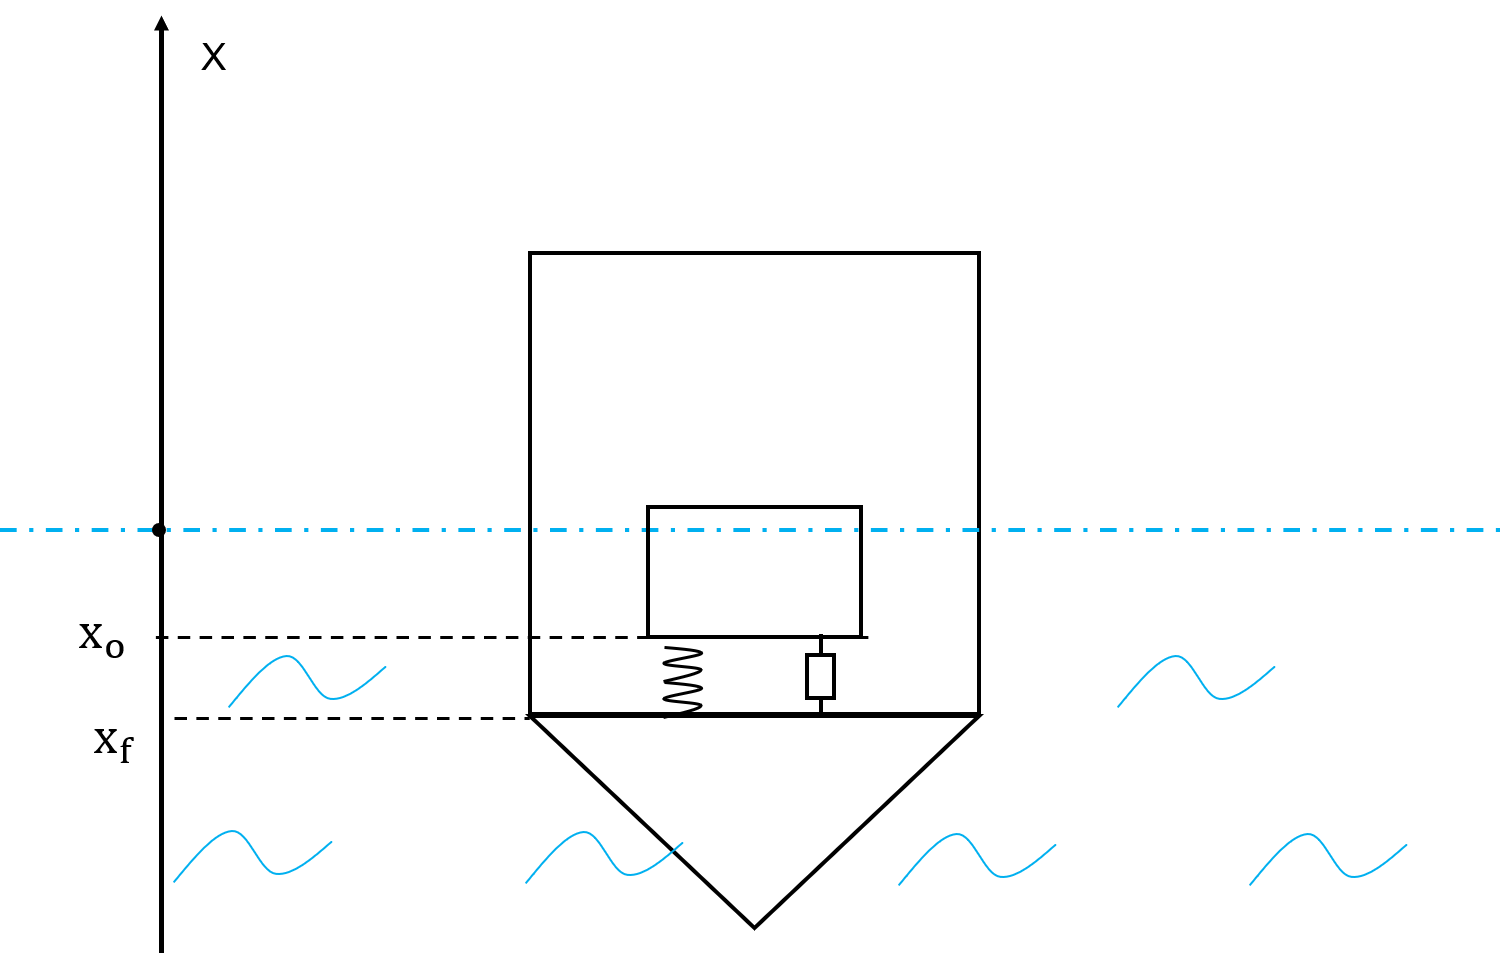
\includegraphics[width=0.6\textwidth]{建系.png}
        \caption[]{一维坐标系}
\end{figure}

\newpage
问题一采用中轴与中轴底座的焦点和中轴振子的下表面的焦点对应的坐标来分别表示振子和浮子的位置。初始时刻浮子和振子的坐标分别为$x_{f}(0)$和$x_{o}(0)$。


\subsubsubsection{对浮子受力分析}

问题一中考虑浮子在波浪中只做垂荡运动。基于假设3,浮子受到的力有波浪激励力、附加惯性力、兴波阻尼力、静水恢复力和PTO对浮子的作用力。


\textbf{1)波浪激励力}

在问题一和问题二中,波浪激励力始终沿着浮子垂荡运动的方向,在题干中波浪激励力以余弦的形式给出,即:
\begin{equation}
    F_w=f\cos wt\label{Q1fbolanjilili}
\end{equation}
其中$w$为入射波浪频率,$f$为波浪激励力振幅。

\textbf{2)附加惯性力}

浮子在海水中做垂荡运动时,会引起周围流体的运动,由于流体具有惯性,表现为对浮子的一个反作用力,称为附加惯性力。附加惯性力对应产生一个虚拟的质量,称为垂荡附加质量。附加惯性力的表达式为:
% 附加惯性力来自辐射力,具体来说是因为还需要推动浮子周围的流体运动而产生的额外的力,可利用附加质量、通过牛顿第二定律得出:
\begin{equation}
    F_a=-m_{a}\ddot x_{f}\label{Q1ffujiaguanxingli}
\end{equation}
其中$m_{a}$为垂荡附加质量,$\ddot x_{f}$为浮子做垂荡运动的加速度。

\textbf{3)兴波阻尼力}

浮子在海水中做垂荡运动时,会产生波浪,从而产生对浮子垂荡运动的阻力,称为兴波阻尼力。兴波阻尼力的大小正比于浮子做垂荡运动的速度,比例系数称为行波阻尼系数。兴波阻尼力的表达式为:
\begin{equation}
    F_{wd}=-c_{h}\dot x_{f}\label{Q1fxingbozunili}
\end{equation}
其中$c_{h}$为垂荡兴波阻尼系数,$\dot x_{f}$为浮子做垂荡运动的速度。

\textbf{4)静水恢复力}

浮子在海水中做垂荡运动时,会受到使浮子重新保持在平时位置的力,称为静水恢复力。它是浮子的重力与所受到的海水浮力的差\cite{黄秀秀2019振荡浮子式波浪发电系统的功率控制}。静水恢复力的表达式为:
\begin{equation}
    F_{HS}=F_{b}-m_{f}g\label{Q1fjingshuihuifuli}
\end{equation}
其中,$F_{b}$为浮子所受到的海水的浮力,$m_{f}$为浮子重量。

浮子在海水中做垂荡运动时受到的海水的浮力为:
\begin{equation}
    F_{b}=\rho g V \label{Q1ffuli}
\end{equation}
其中,$\rho$为海水密度,$g$为重力加速度,$V$为浮子的排水量。

浮子的排水量为:
\begin{equation}\label{Q1fpaishuiliang}
    V=\left\{\begin{matrix}
    0,\quad & x_{f}>0.8 \\
    \frac{1}{3}\pi R_{f}^{2}\frac{(H_{f1}-x_{f})^{3}}{H_{f1}^{2}} & 0<x_{f}\leq 0.8 \\
    \frac{1}{3}\pi R_{f}^{2}H_{f1}-\pi R_{f}^{2}x_{f} & -3<x_{f}\leq 0 \\
    \frac{1}{3}\pi R_{f}^{2}H_{f1}+\pi R_{f}^{2}H_{f2} & x_{f}\leq -3 \\
    \end{matrix}\right.
\end{equation}
其中,$R_{f}$为浮子底半径,$H_{f1}$为浮子圆柱部分高度,$H_{f2}$为浮子圆锥部分高度。

\textbf{5)PTO对浮子的作用力}

能量输出系统PTO包括弹簧和阻尼器。PTO对浮子的作用力是一个与浮子和振子的相对速度成比例的阻尼力和一个与浮子和振子的相对位移成正比的弹簧弹力的合力,即:
\begin{equation}\label{Q1fPTO}
    % F_{PTO}=F_{d}+F_{s}\label{F_PTO}
    % F_{PTO}=-k_{s}\Delta l+c_{s}\Delta\dot x \label{F_PTO}
    \left\{\begin{matrix}
    F_{PTO}=F_{d}+F_{s}  \\
    F_{d}=c_{s} v_{r}  \\
    F_{s}=-k_{s}\Delta l  \\ 
    v_{r}=\dot x_{o}-\dot x_{f} \\
    \Delta l=l_{0}-\Delta x \\
    \Delta x=x_{o}-x_{f} \\
    \end{matrix}\right.
\end{equation}
其中$F_{d}$为直线阻尼器的阻尼力,$F_{s}$为弹簧的弹力,$c_{s}$为直线阻尼器的阻尼系数,$v_{r}$为振子相对于浮子的速度,$k_{s}$为弹簧刚度,$\Delta l$为弹簧形变量,$\Delta x$为振子与浮子的相对位移。

\subsubsubsection{对振子受力分析}

振子被密封在浮子的内部,通过PTO与浮子隔层上的中轴底座相连。通过分析,振子受到重力和PTO系统对它的作用力。

\textbf{1)重力}

振子受到的重力表达式为:
\begin{equation}\label{gravity of o}
    G_{o}=m_{o}g 
\end{equation}
其中,$m_{o}$为振子的质量。

\textbf{2)PTO对振子的作用力}

PTO系统对浮子和振子的作用力大小相等、方向相反。PTO系统对振子的作用力的表达式为:
\begin{equation}\label{PTO force to o}
    F_{PTO}^{'}=-F_{PTO} 
\end{equation}

\newpage
\subsubsection{模型建立}

\subsubsubsection{初始状态的求解}

建立浮子与振子的运动模型前,先对浮子与振子的初始状态进行分析。

初始时刻,整个波浪能装置处于平衡状态,即所受到的合外力为$0$。整个波浪能装置,受到重力和海水对它的浮力作用,并且两者大小相等,方向相反,作用与一条直线上,即:
\begin{equation}
    F-(m_{f}+m_{o})g=0 \label{entity}
\end{equation}

联立式(\ref{Q1ffuli})、(\ref{Q1fpaishuiliang})、(\ref{entity})解得初始时刻浮子的排水量和吃水深度分别为:
$$
V_{x}=7.121m^3
$$
$$
d=2.8m
$$

对于振子,由于初始时刻,浮子与振子处于平衡状态,两者相对静止。因此,振子受到的阻尼力为0,受到的弹簧弹力与振子的重力大小相同,方向相同。结合式(\ref{gravity of o})和(\ref{PTO force to o})得到:
\begin{equation}
    F_{PTO}^{'}-G_{o}=0
\end{equation}
可得初始状态下弹簧长度为:
$$
l=0.195875m
$$

\subsubsubsection{浮子运动方程}

浮子在波浪激励力$F_w$、附加惯性力$F_a$、兴波阻尼力$F_d$、静水恢复力$F_{HS}$和PTO对浮子的作用力$F_{PTO}$五种力的作用下运动。由牛顿第二定律可以确定浮子的运动方程为:
\begin{equation}
    m_f \ddot x_f = F_w+F_{HS}+F_a+F_d+F_{PTO}
\end{equation}

代入式(\ref{Q1fbolanjilili})、(\ref{Q1ffujiaguanxingli})、(\ref{Q1fxingbozunili})、(\ref{Q1fjingshuihuifuli})、(\ref{Q1ffuli})、(\ref{Q1fpaishuiliang})、(\ref{Q1fPTO})后可得:
\begin{equation}
    m_f\ddot x_f=f \cos wt+\rho g V-m_f g-m_{a}\ddot x_f-c_h \dot x_f-k_s[l_0-(x_o-x_f)]+c_s(\dot x_o-\dot x_f)
\end{equation}

\subsubsubsection{振子运动方程}

振子仅受PTO的作用力$F_{PTO}^{'}$和自身重力$G_o$的作用。
由牛顿第二定律得振子的运动方程:
\begin{equation}
    F_{PTO}^{'}-G_o=m_o\ddot x_o\label{Q1oyundongfangcheng}
\end{equation}
由式(\ref{Q1fPTO})、(\ref{gravity of o})、(\ref{PTO force to o})、(\ref{Q1oyundongfangcheng})可得:
\begin{equation}
    k[l_0-(x_o-x_f)]-c_s(\dot x_o -\dot x_f)-m_o g=m_o\ddot x_o
\end{equation}

\subsubsubsection{模型汇总}

综上所述得到浮子与振子的运动模型:
\begin{equation}
    \left\{\begin{matrix} 
        m_f\ddot x_f=f \cos wt+\rho g V-m_f g-m_{a}\ddot x_f-c_h \dot x_{f}-k[l_{0}-(x_{o}-x_{f})]+c_{s}(\dot x_{o}-\dot x_{f}) \\ 
        k_{s}[l_{0}-(x_{o}-x_{f})]-c_{s}(\dot x_{o}-\dot x_{f})-m_{o} g=m_{o}\ddot x_{o} \\  
        x_f(0)=-2, \quad x_{o}(0)=-1.8, \quad x_{o}(0)-x_{f}(0)=0.2\\
        \dot x_f(0)=0, \quad \dot x_o(0)=0\\
  \end{matrix}\right.    \label{bian liang dai huan}
\end{equation}

 \subsubsection{模型求解}

求解此二阶微分方程数值解时,首先做变量替换,将其化为一阶微分方程组,令:
\begin{equation}
        p_1=x_f,\quad p_2=\dot x_f,\quad_3=x_o,\quad p_4=\dot x_o\\
\end{equation}
则二阶微分方程组(\ref{bian liang dai huan})可化为如下的一阶微分方程组:
\begin{equation}
    \left\{\begin{matrix} 

        \dot p_1=p_2, \vspace{1ex} & p1(0)=-2\\ 
        \displaystyle \dot p_2=\frac{-(c_h+c_s)p_{2}-k_s p_{1} + c_s p_{4}+k_s p_{3} - k_s l_{0}+\rho g V-m_{f}g+f \cos wt}{m_{f}+m}, \vspace{1ex} &p2(0) = 0\\  
        \dot p_3=p_4,\vspace{1ex} & p3(0)=-1.8\\
        \displaystyle\dot p_4=\frac{c_{s} p_{4}+k_{s} p_{3}-c_{s} p_{2}-k_{s} p_{1}+m_{o}g-k_{s} l_{0}}{-m_{o}}, & p4(0)=0\\
  \end{matrix}\right.    
\end{equation}

使用Matlab工具箱中的ode45函数(采用四五阶龙格-库塔算法)\cite{司守奎2007数学建模算法与程序},分别求解该微分方程在$c_{s}=10000N\cdot s/m$与$c_{s}=10000 \lvert v_{r} \rvert^\frac{1}{2}N\cdot s/m$
时的数值解。
\subsubsection{结果分析}

\noindent
\textbf{(1)阻尼系数为常数,即$c_s=10000N\cdot m$}

浮子与振子的位移随时间变化图像如图2和3所示。
\newpage

\begin{figure}[!ht]
    \centering
    \begin{minipage}[t]{0.48\textwidth}
    \centering
    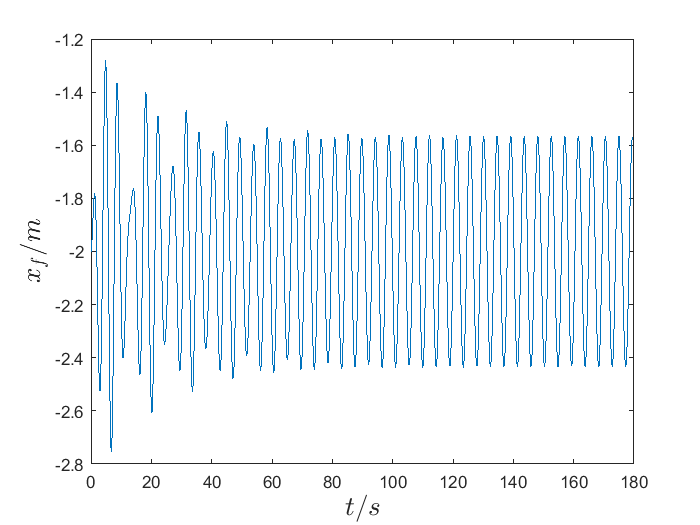
\includegraphics[width=8cm]{1-1f.png}
    \caption{浮子位移-时间关系图}
    \end{minipage}
    \begin{minipage}[t]{0.48\textwidth}
    \centering
    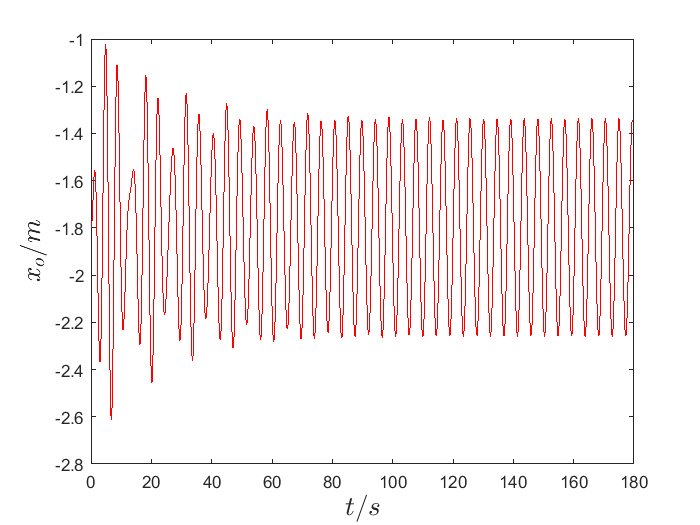
\includegraphics[width=8cm]{1-1o.png}
    \caption{振子位移-时间关系图}
    \end{minipage}
    \end{figure}

从图2、图3中可以看出浮子和振子在经历一小段的不规则震荡之后,开始进行周期性的
运动,其中振子在-1.8米左右做周期运动,浮子在-2米左右做周期运动。
浮子和振子在10s、20s、40s、60s、100s的垂荡位移与速度如表1所示:
% Please add the following required packages to your document preamble:
% \usepackage{multirow}
\begin{table}[!h]
    \centering
        \setlength{\belowcaptionskip}{0.2cm}
      \caption{浮子、振子速度位移表Ⅰ}
    \begin{tabular}{|c|cc|cc|}
    \hline
    \multirow{2}{*}{\textbf{时间 (s)}} & \multicolumn{2}{c|}{\textbf{浮子}}                         & \multicolumn{2}{c|}{\textbf{振子}}                         \\ \cline{2-5} 
                                     & \multicolumn{1}{c|}{\textbf{位移 (m)}} & \textbf{速度 (m/s)} & \multicolumn{1}{c|}{\textbf{位移 (m)}} & \textbf{速度 (m/s)} \\ \hline
    10                               & \multicolumn{1}{c|}{-2.190954076}    & -0.640777992      & \multicolumn{1}{c|}{-2.01000313}    & -0.693713854      \\ \hline
    20                               & \multicolumn{1}{c|}{-2.590791425}    & -0.240503252      & \multicolumn{1}{c|}{-2.43236668}     & -0.272701067      \\ \hline
    40                               & \multicolumn{1}{c|}{-1.714640468}    & 0.313200313       & \multicolumn{1}{c|}{-1.501579719}    & 0.333354995       \\ \hline
    60                               & \multicolumn{1}{c|}{-2.314474968}    & -0.479244744      & \multicolumn{1}{c|}{-2.129483735}    & -0.515476772      \\ \hline
    100                              & \multicolumn{1}{c|}{-2.083607248}    & -0.604068126      & \multicolumn{1}{c|}{-1.882096565}    & -0.643048215      \\ \hline
    \end{tabular}
  
    \end{table}


\noindent\textbf{(2)阻尼系数与浮子和振子的相对速度的绝对值的幂成正比
,即$c_s=10000N\cdot m$,$c_{s}=10000 \lvert v_{r} \rvert^{0.5} N\cdot s/m$。}

浮子与振子的位移随时间变化如图4和5所示。
从图4、图5中可以看出此时浮子与振子的运动变化趋势与情况(1)中相似,一段时间
震荡后振子在-1.8m处做周期垂荡运动,浮子在-2m处做周期垂荡运动。


\begin{figure}[!htbp]
    \centering
    \begin{minipage}[t]{0.48\textwidth}
    \centering
    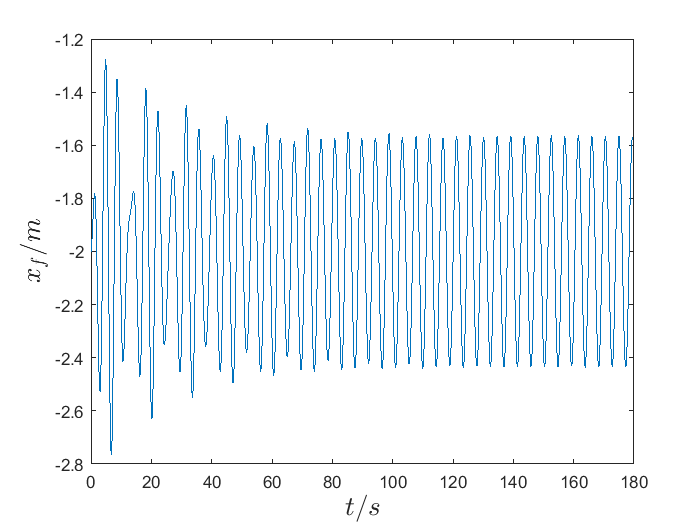
\includegraphics[width=8cm]{1-2f.png}
    \caption{浮子位移-时间关系图}
    \end{minipage}
    \begin{minipage}[t]{0.48\textwidth}
    \centering
    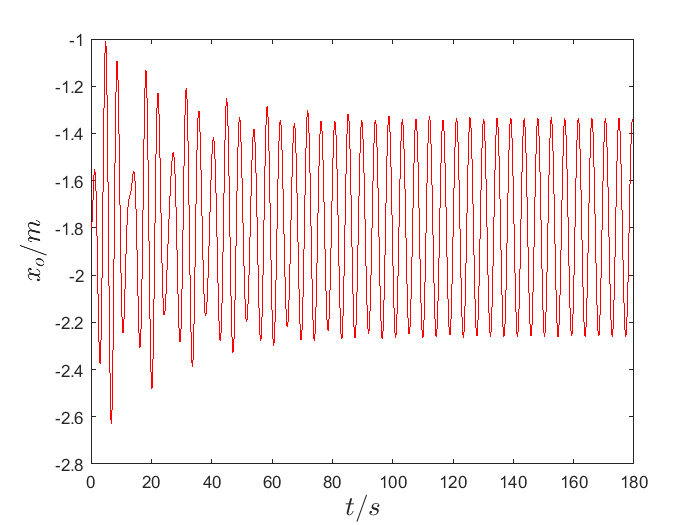
\includegraphics[width=8cm]{1-2o.png}
    \caption{振子位移-时间关系图}
    \end{minipage}
    \end{figure}
\newpage

浮子和振子在10s、20s、40s、60s、100s的垂荡位移与速度如表2所示:
% Please add the following required packages to your document preamble:
% \usepackage{multirow}
\begin{table}[!h]
    \setlength{\belowcaptionskip}{0.2cm}
    \caption{浮子、振子速度位移表Ⅱ}
    \centering
    \begin{tabular}{|c|cc|cc|}
    \hline
    \multirow{2}{*}{\textbf{时间 (s)}} & \multicolumn{2}{c|}{\textbf{浮子}}                         & \multicolumn{2}{c|}{\textbf{振子}}                         \\ \cline{2-5} 
                                     & \multicolumn{1}{c|}{\textbf{位移 (m)}} & \textbf{速度 (m/s)} & \multicolumn{1}{c|}{\textbf{位移 (m)}} & \textbf{速度 (m/s)} \\ \hline
    10                               & \multicolumn{1}{c|}{-2.20624292}     & -0.652613932      & \multicolumn{1}{c|}{-2.033048486}    & -0.699040381      \\ \hline
    20                               & \multicolumn{1}{c|}{-2.61129173}     & -0.254065041      & \multicolumn{1}{c|}{-2.459200861}    & -0.276577707      \\ \hline
    40                               & \multicolumn{1}{c|}{-1.731431789}    & 0.295841034       & \multicolumn{1}{c|}{-1.517986272}    & 0.314112722       \\ \hline
    60                               & \multicolumn{1}{c|}{-2.32719546}     & -0.491221073      & \multicolumn{1}{c|}{-2.147706499}    & -0.52409872       \\ \hline
    100                              & \multicolumn{1}{c|}{-2.088343237}    & -0.609417569      & \multicolumn{1}{c|}{-1.891710692}    & -0.650329169      \\ \hline
    \end{tabular}
 
    \end{table}


% 看图说话,对结果进行分析!!!!!!!!!!!!!!!!!!!!!!!!!!!
%!!!!!!!!!!!!!!!!!!!!!!!!!!!!!!!!!!!!!!!!!



\subsection{问题二}

\subsubsection{模型建立}

\textbf{Step 1 优化目标}

浮子与振子的相对运动驱动阻尼器做功,并将所做作为能量输出。波浪能装置的瞬时功率为\cite{oskamp2012power}:
\begin{equation}
    P=F_{d} v_{r}\label{average Power}
\end{equation}
其中$v_{r} $为振子相对于浮子的速度。

由式(\ref{Q1fPTO})、(\ref{average Power})可得:
\begin{equation}
    P=c_{s} v_{r}^2\label{shunshigonglv}
\end{equation}

平均输出功率为:
\begin{equation}
    \overline{P}=\frac{1}{T}\int_{0}^{T}{P}\,{\rm d}t\label{pingjungonglv}
\end{equation}

根据问题二,需要求解设定阻尼系数下允许的PTO系统最大平均输出功率,则目标为平均输出功率最大。结合式(\ref{shunshigonglv})、(\ref{pingjungonglv}),优化目标为:

$$
\max \quad \overline{P}=\frac{1}{T}\int_{0}^{T}{c_{s} v_{r}^2}\,{\rm d}t
$$

\textbf{Step 2 约束条件}

根据题目信息,约束条件为阻尼系数。

\noindent
\textbf{(1)} 阻尼系数为常量
        \begin{equation}
            0\leq c_{s}\leq 100000
        \end{equation}        
\noindent
\textbf{(2)} 阻尼系数与浮子和振子的相对速度的绝对值的幂成正比
        \begin{equation}
            \left\{\begin{matrix}
            c_{s}=\sigma \lvert v_{r}\rvert^r \\
            0\leq \sigma\leq 100000 \\
            0\leq r\leq 1 \\
            
            \end{matrix}\right.
        \end{equation}
        其中,$\sigma$为比例系数,$r$为幂指数。
    

\textbf{Step 3 模型综合}

综上所述,建立最优阻尼系数的输出功率模型综合如下:

    \textbf{(1)} 阻尼系数为常量
        \begin{equation}
            \left\{\begin{matrix}
                \max & \overline{P}=\frac{1}{T}\int_{0}^{T}{c_{s} v_{r}^2}\,{\rm d}t\\
                s.t. & 0 \leq c_s\leq 100000 \\
                    &  m_f \ddot x_f = F_w+F_{HS}+F_a+F_d+F_{PTO}\\
                    &  F_{PTO}^{'}-G_o=m_o\ddot x_o\\
            \end{matrix}
            \right.
        \end{equation}
        


    \textbf{(2)} 阻尼系数与浮子和振子的相对速度的绝对值的幂成正比
        
        \begin{equation}
            \left\{\begin{matrix}
                \max & \overline{P}=\frac{1}{T}\int_{0}^{T}{c_{s} v_{r}^2}\,{\rm d}t\\
                s.t. & c_{s}=\sigma \lvert v_{r}\rvert^r\\
                    & 0\leq \sigma\leq 100000 \\
                    & 0\leq r\leq 1 \\ 
                    &  m_f \ddot x_f = F_w+F_{HS}+F_a+F_d+F_{PTO}\\
                    &  F_{PTO}^{'}-G_o=m_o\ddot x_o\\
            \end{matrix}
            \right.
        \end{equation}


\subsubsection{模型求解}

求解平均功率计算式中所需的$v_{i}$,需结合第一问中所建立的浮子、振子的运动模型,将浮子、振子的运动方程与两种情况下的平均功率计算式、约束条件结合后可得最终的目标优化方程组

\noindent\textbf{(1)阻尼系数为常量时:}
\begin{equation}
            \left\{\begin{matrix}
                \max & \overline{P}=\frac{1}{T}\Sigma{c_{s} v_{r}^2 \Delta t}\\
                s.t. & 0 \leq c_s\leq 100000 \\
                    &  m_f \ddot x_f = F_w+F_{HS}+F_a+F_d+F_{PTO}\\
                    &  F_{PTO}^{'}-G_o=m_o\ddot x_o\\
            \end{matrix}
            \right.
        \end{equation}

\noindent\textbf{(2)阻尼系数与$v_r$的绝对值的幂成正比时:}
\begin{equation}
    \left\{\begin{matrix}
       \max & \overline{P}=\frac{1}{T}\Sigma{c_{s} v_{r}^2 \Delta t}\\
        s.t. & c_{s}=\sigma \lvert v_{r}\rvert^r\\
            & 0\leq \sigma\leq 100000 \\
            & 0\leq r\leq 1 \\ 
            &  m_f \ddot x_f = F_w+F_{HS}+F_a+F_d+F_{PTO}\\
            &  F_{PTO}^{'}-G_o=m_o\ddot x_o\\
    \end{matrix}
    \right.
\end{equation}


使用粒子群算法求解。
粒子群算法(PSO)是一种于1995年提出的进化算法,其基本思想是通过群体中每个个体的信息共享与协作来寻找最优的解,其基本的算法步骤如下:\\

\begin{tabular}{l}
   
   \toprule
    \toprule
    
    \textbf{Step 1:}  初始化一群数量为N粒子,同时随机设定他们的位置和速度 \\
  
    \textbf{Step 2;}  计算每一个粒子的适应度\\
  
    \textbf{Step 3;}  更新粒子个体最优值\\
  
    \textbf{Step 4;}  更新粒子群体最优值\\
  
    \textbf{Step 5;}  判断是否符合最优或者达到最大迭代次数,若都没达成,跳转步骤7,否则进入步骤6\\
  
    \textbf{Step 6;} 依据个体最优值和群体最优值更新各粒子的位置和速度,重复3、4、5三个步骤\\
  
    \textbf{Step 7:} 输出结果,结束算法
  \\
    \midrule
  \end{tabular}
 

取$\Delta t = 0.10s$,

\noindent\textbf{(1)阻尼系数为常量时:}
\begin{equation}
    \overline{P}_{max}=246.118W\, \quad C=37667.1025  
\end{equation}

\noindent\textbf{(2)阻尼系数与$v_r$的绝对值的幂成正比时:}
\begin{equation}
    \overline{P}_{max}=1216.1029W\, \quad \sigma=99643.3182\, \quad r=1  
\end{equation}


\subsection{问题三}
\subsubsection{模型准备}
\begin{figure}[!htbp]
    \centering
    \begin{minipage}[t]{0.48\textwidth}
    \centering
    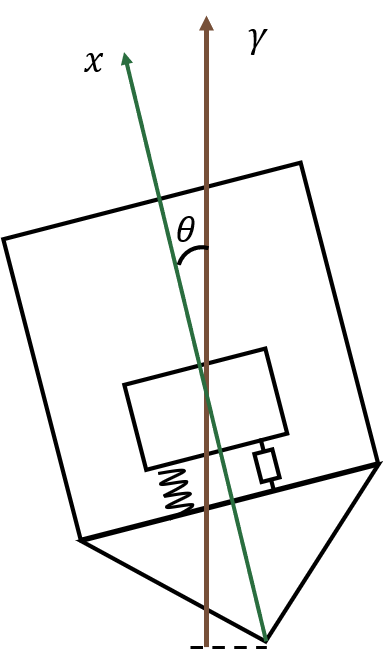
\includegraphics[width=0.5\textwidth]{轴2.png}
    \label{zhou two}
    \caption{坐标系的建立}
    \end{minipage}
    \begin{minipage}[t]{0.48\textwidth}
    \centering
    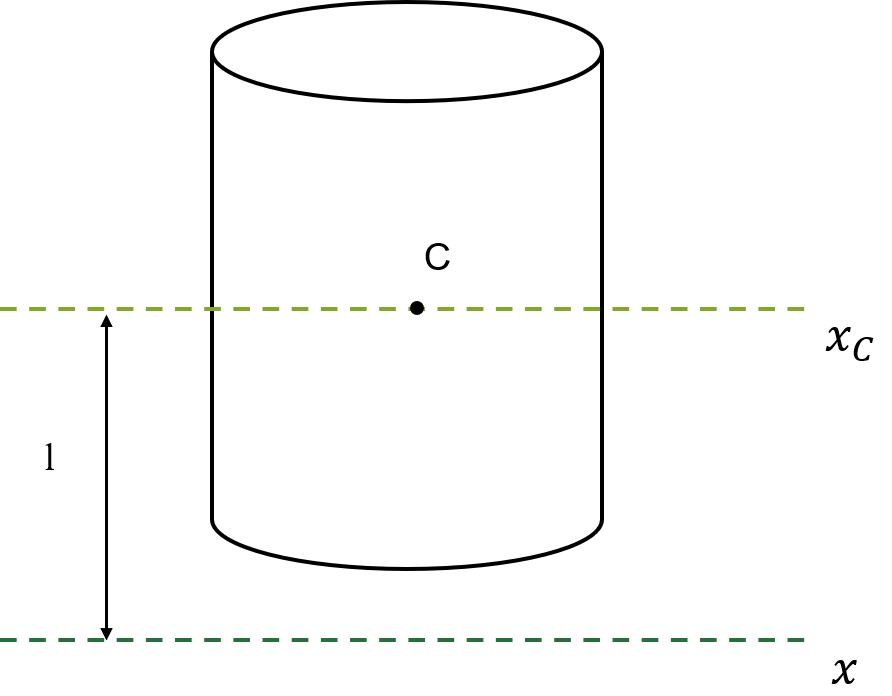
\includegraphics[width=0.8\textwidth]{圆柱.png}
    \caption{圆柱的转动惯量}
    \end{minipage}
    \end{figure}
    
\subsubsubsection{坐标系的建立}

以初始时刻的中轴与海平面的交点为原点,建立坐标系。见图6,$x$表示物体在垂荡方向上的坐标,$\theta$表示物体在纵摇方向上偏离$\gamma$轴的角度,规定物体沿$x$轴为正方向,规定物体逆时针转动方向为正方向。

在问题三与问题四中,定义$x_{f}$为浮子隔层圆心的坐标,$x_{o}$为振子下表面圆心的坐标,$\theta_{f}$为浮子偏离$\gamma$轴的角度,$\theta_{o}$为振子偏离$\gamma$轴的角度。

\subsubsubsection{平行轴定理}

    在已知刚体对于一支质心轴的转动惯量,利用平行轴定理能够很简易地计算刚体对平行于质心轴的另外一支轴的转动惯量。
    $$
    I=I_{c}+m d_{x}^{2}
    $$
    其中,$I_{c}$代表刚体对于质心轴的转动惯量,$m$代表刚体的质量,$l$代表另外一支与质心轴平行的直轴与质心轴的垂直距离。

\subsubsubsection{转动惯量的计算}


\textbf{1)两端开通的圆柱壳体的转动惯量}


两端开通的薄圆柱壳对如图7中通过其质心的轴$X_c$的转动惯量为:

\begin{equation}
    I_c=\frac{1}{2}m r^{2}+\frac{1}{12}m h^{2}
\end{equation}

其中$m$为圆柱薄壳质量,$r$为圆柱薄壳半径,$h$为圆柱薄壳高度。

设另有一轴$X$与$X_c$平行,且距离轴$X_c$为L,则通过平行轴定理可知该刚体
对于轴$X$的转动惯量为:
\begin{equation}
    I=\frac{1}{2}m r^{2}+\frac{1}{12}m H^2+m l^2 \label{yuanzhuqiao}
\end{equation}

\textbf{2)浮子的转动惯量}

\begin{figure}[!h]
    \centering
    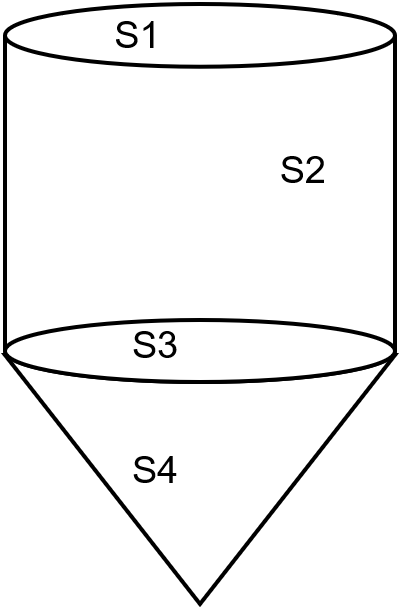
\includegraphics[width=0.25\textwidth]{四面.png}
    \caption{浮子的四个面}
    \label{fig:my_label}
\end{figure}
浮子由圆锥壳体和圆柱壳体组成,如图8,可分为四个面,从上至下依次命名为$S_1$、$S_2$、$S_3$、$S_4$。
$S_1$的转动惯量为:
\begin{equation}
    I_{f1}=\frac{1}{4}m_{f1}R_f^{2}+m_{f1}H_{f1}^2
    \label{mian 1}
\end{equation}
根据式(\ref{yuanzhuqiao}),$S_2$的转动惯量为:
\begin{equation}
    I_{f2}=\frac{1}{2}m_{f1} R_f^{2}+\frac{1}{12}m_{f3} H_{f1}^2+m_{f3}(\frac{H_{f1}}{2})^2
    \label{mian 1}
\end{equation}
$S_3$关于转轴的
转动惯量为:
\begin{equation}
I_{f3}=\frac{1}{4}m_{f3}R_f^{2}\label{mian 3}
\end{equation}
其中$m_{f1}$,$m_{f2}$,$m_{f3}$,$m_{f4}$根据对应的面积占比来计算,因为浮子的质量式均匀分布的。
面$S_4$的转动惯量$I_{f4}$可通过微元的方法求出(详细的推倒过程在附录中给出):


浮子的转动惯量为:
\begin{equation}
    I_{f} = I_{f1} + I_{f2} + I_{f3} + I_{f4}
\end{equation}

\textbf{3)实心圆柱转动惯量}

实心圆柱对如图7中通过其质心的轴$X_c$的转动惯量为:

\begin{equation}
    I_c=\frac{1}{12}m (3r^{2} + h^2)
\end{equation}
其中$m$为刚体质量,$r$为刚体半径,$h$为刚体高度

设另有一轴$X$与$X_c$平行,且距离轴$X_c$为$d_{x}$,则通过平行轴定理可知该刚体
对于轴$X$的转动惯量为:
\begin{equation}\label{37}
    I=\frac{1}{12}m (3r^{2} + h^2)+m d_{x}^2
\end{equation}


\textbf{4)浮子转动惯量}

由式(\ref{37})即可求得振子对转轴的转动惯量:

\begin{equation}
    I_o=\frac{1}{12}m_o (3R_o^{2} + H_o^2)+m_o(x_o-x_f+\frac{H_o}{2})^2
\end{equation}

\subsubsubsection{垂荡运动时的对浮子受力分析}

在问题三中,考虑浮子只做垂荡运动和纵摇运动。因此,需要在问题一中对浮子与振子的受力分析的基础上,考虑浮子与振子受到的力矩作用以及垂荡运动和纵摇运动间的耦合关系。因此,在考虑浮子只做垂荡运动和纵摇运动之前,先考虑浮子只做纵摇运动的情况下浮子和振子的运动模型\cite{周丙浩2018纵摇浮子式波浪能转换装置研究}。


\textbf{1)波浪激励力矩}

在问题三中,波浪激励力矩始终沿着浮子纵摇运动的方向,波浪激励力矩以余弦的形式给出,即:
\begin{equation}
    M_w=L\cos wt\label{Q3fbolanjililiju}
\end{equation}
其中$w$为入射波浪频率,$L$为波浪激励力矩振幅。


\textbf{2)附加惯性力矩}

浮子在海水中做纵摇运动时,会引起周围流体的运动,由于流体具有惯性,表现为对浮子的一个反作用力矩,称为附加惯性力矩。附加惯性力矩对应产生一个虚拟转动惯量,称为纵摇附加转动惯量。附加惯性力矩的表达式为:
% 附加惯性力来自辐射力,具体来说是因为还需要推动浮子周围的流体运动而产生的额外的力,可利用附加质量、通过牛顿第二定律得出:
\begin{equation}
    M_a=-I_{a}\ddot \theta_{f}\label{Q3ffujiaguanxingliju}
\end{equation}
其中$I_{a}$为纵摇附加质量,$\ddot \theta_{f}$为浮子做纵摇运动的加速度。

\textbf{3)兴波阻尼力矩}

浮子在海水中做纵摇运动时,会产生波浪,从而产生对浮子纵摇运动的阻力矩,称为兴波阻尼力矩。兴波阻尼力矩的大小正比于浮子做纵摇运动的速度,比例系数称为行波阻尼系数。兴波阻尼力矩的表达式为:
\begin{equation}
    M_{wd}=-c_{p}\dot \theta_{f}\label{Q3fxingbozuniliju}
\end{equation}
其中$c_{p}$为纵摇兴波阻尼系数,$\dot \theta_{f}$为浮子做纵摇运动的速度。

\textbf{4)静水恢复力矩}

浮子在海水中做纵摇运动时,会受到使其转正的力矩,称为静水恢复力矩。静水恢复力矩的大小与$\theta_{f}$成正比,表达式为:
\begin{equation}
    M_{HS}=-K_{HS}\theta_{f}\label{Q3jingshuihuifuliju}
\end{equation}
其中,$K_{HS}$为静水恢复力矩系数。

\textbf{5)PTO对浮子的作用力矩}

能量输出系统PTO包括弹簧和阻尼器。PTO对浮子的作用力矩是一个与浮子和振子的相对速度成比例的阻尼力矩和一个与浮子和振子的相对位移成正比的弹簧弹力矩的合力矩,即:
\begin{equation}\label{Q3fPTO}
    % F_{PTO}=F_{d}+F_{s}\label{F_PTO}
    % F_{PTO}=-k_{s}\Delta l+c_{s}\Delta\dot x \label{F_PTO}
    \begin{cases}
    M_{PTO}=M_{d}+M_{s}  \\
    M_{d}=c_{t}w_{r}  \\
    M_{s}=k_{t}\Delta \theta  \\ 
    w_{r}=\dot \theta_{o}-\dot \theta_{f} \\
    \Delta \theta=\theta_{o}-\theta_{f} \\
    \end{cases}
\end{equation}
其中$M_{d}$为旋转阻尼器的旋转阻尼力矩,$M_{t}$为弹簧的弹力矩,$c_{t}$为直线旋转阻尼器的旋转阻尼系数,$w_{r}$为振子相对于浮子的角速度,$k_{t}$为扭转弹簧刚度,$\Delta \theta$为振子与浮子的相对角位移。


\subsubsubsection{垂荡运动时的对振子受力分析}

振子被密封在浮子的内部,通过PTO和转轴架与浮子隔层上的中轴底座相连。振子受到重力矩和PTO系统对它的作用力矩。

\textbf{1)重力矩}

振子受到的重力矩表达式为:
\begin{equation}\label{Q3ozhongliju}
    M_{G}=m_{o}g\sin{\theta_{o}}\cdot (\frac{1}{2}H_{o}+\Delta x)^2 
\end{equation}
其中,$m_{o}$为振子的质量。

\textbf{2)PTO对振子的作用力矩}

PTO系统对浮子和振子的作用力矩大小相等、方向相反。PTO系统对振子的作用力矩的表达式为:
\begin{equation}\label{Q3oPTO}
    M_{PTO}^{'}=-M_{PTO}
\end{equation}



\subsubsection{模型建立}

\subsubsubsection{浮子只做纵摇运动时的运动方程}

    \textbf{1)浮子的运动方程}
    
    考虑浮子只做纵摇运动时,浮子受到波浪激励力矩$M_{w}$、附加惯性力矩$M_{a}$、兴波阻尼力矩$M_{wd}$、静水恢复力矩$M_{HS}$、PTO对的作用力矩$M_{PTO}$的作用。由牛顿第二定律可以确定浮子的运动方程为:
    \begin{equation}
        I_{f} \ddot \theta_{f} = M_w+M_{HS}+M_a+M_{Wd}+M_{PTO}
    \end{equation}
    
    由式(\ref{Q3fbolanjililiju})、(\ref{Q3ffujiaguanxingliju})、(\ref{Q3fxingbozuniliju})、(\ref{Q3jingshuihuifuliju})、(\ref{Q3fPTO})得:
    \begin{equation}
      I_f\ddot \theta_{f}=L\cos wt -I_a\ddot \theta_{f}-c_p\dot \theta_{f}-K_{HS}\theta_{f}+k_t(\theta_{o}-\theta_{f})+c_t(\dot\theta_{o}-\dot\theta_{f})
    \end{equation}
    
    \textbf{2)振子的运动方程}
    
    考虑浮子只做纵摇运动时,振子受到PTO的作用力矩$M_{PTO}$和重力分力提供的力矩。由牛顿第二定律可以确定振子的运动方程为:
    \begin{equation}
        I_{o} \ddot \theta_{o} = M_{PTO}^{'}+M_{G}
    \end{equation}
    
    由式(\ref{Q3oPTO})、(\ref{Q3ozhongliju})得:
    \begin{equation}
        I_o\ddot\theta_{o}=-k_t(\theta_o-\theta_f)-ct(\dot\theta_o-\dot\theta_f)+m_og\sin \theta_{o}(\frac{1}{2}H_o+l_0)        
    \end{equation}

\subsubsubsection{考虑浮子只做垂荡运动}

    考虑浮子只做垂荡运动时,浮子与振子的运动模型如下:
    \begin{equation}
        \left\{\begin{matrix} 
            m_f\ddot x_f=f \cos wt+\rho g V-m_f g-m_{a}\ddot x_f-c_h \dot x_{f}-k_s[l_{0}-(x_{o}-x_{f})]+c_{s}(\dot x_{o}-\dot x_{f}) \\ 
           m_{o}\ddot x_{o}= k_{s}[l_{0}-(x_{o}-x_{f})]-c_{s}(\dot x_{o}-\dot x_{f})-m_{o}g\\  
            x_f(0)=-2, \quad x_{o}(0)=-1.8, \quad x_{o}(0)-x_{f}(0)=0.2\\
            \dot x_f(0)=0, \quad \dot x_o(0)=0\\
        \end{matrix}\right.    
    \end{equation}
    
\subsubsubsection{考虑浮子只做纵摇运}

    考虑浮子只做纵摇运动时,浮子与振子的运动模型如下:
    \begin{equation}
    \left\{\begin{matrix}
        I_f\ddot\theta_{f}=L\cos wt -I_a\ddot\theta_{f}-c_p\dot\theta_{f}-K_{HS}\theta_{f}+k_t(\theta_{o}-
    \theta_{f})+c_t(\dot\theta_{o}-\dot\theta_{f})\\
    I_o\ddot\theta_{o}=-k_t(\theta_o-\theta_f)-ct(\dot\theta_o-\dot\theta_f)+m_og\sin \theta_{o}(\frac{1}{2}H_o+l_0)\\
    \theta_{f} (0)=0 \quad \theta_{0}(0)=0\\
    \dot\theta_{f} (0)=0 \quad \dot\theta_{0}(0)=0\\
    
    \end{matrix}\right.
    \end{equation}

\subsubsubsection{考虑垂荡运动和纵摇运动的耦合关系}

    \textbf{1)考虑耦合关系对于浮子运动的影响}
    
        考虑浮子同时做垂荡和纵摇运动,浮子和振子在沿中轴方向运动的同时,与海平面会有一个角度的偏移。浮子与振子的相对角位移使得PTO系统对浮子作用力$F_{PTO}$的方向发生变化,而振子的角度偏离于平衡状态使得浮子受到一个反重力矩$M_{a}$。
        
        通过上述分析,基于浮子垂荡运动和纵摇运动的耦合关系的影响,对浮子的运动模型进行修正,修正后的模型如下:
        % (!!!!!!!)浮子垂荡运动和纵摇运动数学模型+耦合关系
        \begin{equation}
            \left\{\begin{matrix}
                 m_f\ddot x_f=f \cos wt+\rho g V-m_f g-m_{a}\ddot x_f-c_h \dot x_{f}-\{k_s[l_{0}-(x_{o}-x_{f})]+c_{s}(\dot x_{o}-\dot x_{f})\}\cos(\theta_{o}-\theta_{f}) \\
                    I_f\ddot\theta_{f}=L\cos wt -I_o\ddot\theta_{f}-c_p\dot\theta_{f}-K_{HS}\theta_{f}+k_t(\theta_{o}-
    \theta_{f})+c_t(\dot\theta_{o}-\dot\theta_{f})-m_og\sin \theta_{o}(\frac{1}{2}H_o+x_o-x_f) \\
        x_{f} (0)=-2 \quad \dot x_{f}(0)=0\\
    \dot\theta_{f} (0)=0 \quad \dot\theta_{f}(0)=0\\
            \end{matrix}\right.
        \end{equation}
        
        
    \textbf{2)考虑耦合关系对于振子运动的影响}
        
        考虑浮子同时做垂荡和纵摇运动,浮子和振子在沿中轴方向运动的同时,与海平面会有一个角度的偏移。振子与竖直方向夹角的偏移会导致振子在沿中轴方向上的分力大小$mg\cos \theta_{o}$发生变化,同时振子会受到另一个垂直方向上的重力分力提供的力矩$mg\sin \theta \cdot (\frac{1}{2}H_{o}+\Delta x)$。
        
        通过上述分析,基于浮子垂荡运动和纵摇运动的耦合关系的影响,对振子的运动模型进行修正,修正后的模型如下:
        % (!!!!!!!)振子垂荡运动和纵摇运动数学模型+耦合关系  
        \begin{equation}
        \left\{\begin{matrix}
        m_{o}\ddot x_{o}=k_{s}[l_{0}-(x_{o}-x_{f})]-c_{s}(\dot x_{o}-\dot x_{f})-m_{o}\cos \theta_{o} \\  
        I_o\ddot\theta_{o}=-k_t(\theta_o-\theta_f)-ct(\dot\theta_o-\dot\theta_f)+m_og\sin \theta_{o}(\frac{1}{2}H_o+x_o-x_f)\\
        x_o(0)=-1.8, \quad \dot x_{o}(0)=0\\
        \dot \theta_o(0)=0, \quad \dot \theta_o(0)=0\\
        
        \end{matrix}\right.
        \end{equation}
        
\subsubsection{模型求解}

\subsubsubsection{模型综合}

同时进行垂荡运动和纵摇运动的浮子和振子的运动模型如下:
\begin{equation}
    \left\{\begin{matrix}
    m_f\ddot {x}_f=f \cos wt+\rho g V-m_f g-m_{a}\ddot x_f-c_h \dot x_{f}-\{k_s[l_{0}-(x_{o}-x_{f})]+c_{s}(\dot x_{o}-\dot x_{f})\}\cos(\theta_{o}-\theta_{f}) \\
        I_f\ddot\theta_{f}=L\cos wt -I_o\ddot\theta_{f}-c_p\dot\theta_{f}-K_{HS}\theta_{f}+k_t(\theta_{o}-
\theta_{f})+c_t(\dot\theta_{o}-\dot\theta_{f})-mg\sin \theta_{o}(\frac{1}{2}H_o+x_o-x_f) \\
I_o\ddot\theta_{o}=-k_t(\theta_o-\theta_f)-c_t(\dot\theta_o-\dot\theta_f)+m_og\sin \theta_{o}(\frac{1}{2}H_o+x_o-x_f)\\
m_{o}\ddot x_{o}=k_{s}[l_{0}-(x_{o}-x_{f})]-c_{s}(\dot x_{o}-\dot x_{f})-m_{o}\cos \theta_{o} \\  
x_f(0)=-2, \quad x_{o}(0)=-1.8\\
\dot x_f(0)=0, \quad \dot x_o(0)=0\\
\theta_{f} (0)=0 \quad \theta_{o}(0)=0\\
\dot\theta_{f} (0)=0 \quad \dot \theta_{o}(0)=0\\
\end{matrix}\right.
\end{equation}

\subsubsubsection{变量替换}

同样使用龙格-库塔方法求解,故先进行变量替换,令
\begin{equation}
   \left\{\begin{matrix}
       p_1=x_f \quad p_2=\dot x_f  \quad p_3=x_o \quad p_4=\dot x_o\\
       p_5=\theta_{f} \quad p_6=\dot \theta_{f} \quad p_7=\theta_{o} \quad p_8=\dot \theta_{o} \\
   \end{matrix}\right.                                  
\end{equation}

替换后可得
\begin{equation}
      \left\{\begin{matrix}
\displaystyle\dot p_1=p_2     &  p_1(0)=-2 \\
\displaystyle \dot p_2=(f\cos wt-c_hp_2+(\rho gv-m_fg )\cos p_5+ \\
\{-k_s[l_0-(p_3-p_2)+c_s(p_4-p_2)]\}\cos(p_7-p_5))/(m_f+m_{a1})    & p_2(0)=0   \\
\displaystyle\dot p_3=p_4     &  p_3(0)=0 \\[3mm]
\displaystyle\dot p_4=\frac{k_S[l_0-(p_3-p_1)]-c_s(p_4-p_2)-m_o g \cos p_7}{m_o}    & p_4(0)=0 \\
\displaystyle\dot p_5=p_6     & p_5(0)=0  \\[3mm]
\displaystyle\dot p_6= \frac{L\cos wt -c_pp_6-K_{HS}p_5+k_t(p_7-p_5)+c_t(p_8-p_6)}{I_f+I_a}    &  p_6(0)=0 \\
\displaystyle\dot p_7=p_8     & p_7(0)=0  \\[3mm]
\displaystyle\dot p_8=\frac{-kt(p_7-p_5)-c_t(p_8-p_6)+m_og\sin p_7(\frac{1}{2}H_0+p_3-p_1)}{\frac{1}{12}m_o(3R_0^2+H_o^2)+m_o(\frac{1}{2}H_o+p_3-p_1)^2}     & p_8(0)=0  \\
   \end{matrix}\right. 
\end{equation}

使用Matlab工具箱中的ode45求解该微分方程组的数值解。

\subsubsection{结果分析}
求解得到浮子在前四十个波浪周期的垂荡位移与纵摇角位移的变化图像如图9和图10所示。
\newpage


\begin{figure}[!htbp]
    \centering
    \begin{minipage}[t]{0.48\textwidth}
    \centering
    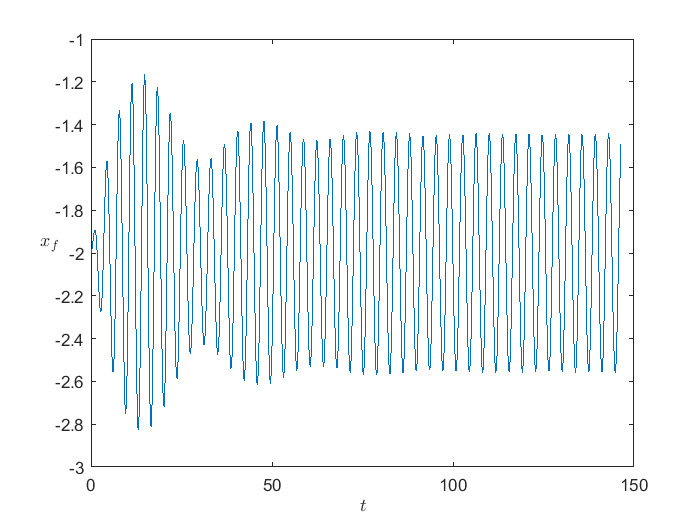
\includegraphics[width=8cm]{3_xf.png}
    \caption{浮子垂荡位移-时间关系图}
    \label{fuzi chui}
    \end{minipage}
    \begin{minipage}[t]{0.48\textwidth}
    \centering
    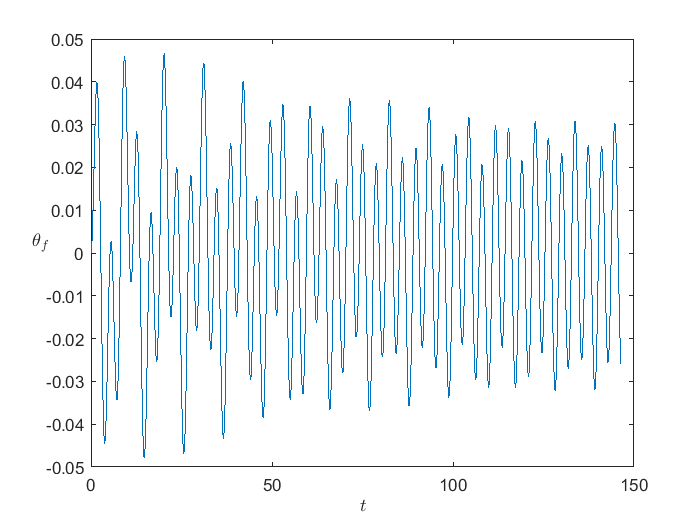
\includegraphics[width=8cm]{3_thetaf.png}
    \caption{浮子纵摇角位移-时间关系图}
   \label{fuzi jiao}
    \end{minipage}
    \end{figure}

振子的在前四十个波浪周期的垂荡位移与纵摇角的位移如图11和图12所示。
由图9、10、11、12可以看出浮子和振子的垂荡位移和纵摇角位移在起初发生
小规模争当变化后逐渐趋于稳定的周期变化,其中浮子的垂荡位移、纵摇角位移变化区间的中值分别为-2$m$,0$rad$;振子的垂荡位移、纵摇角位移变化区间的中值分别为-1.8$m$,0 $rad$;
\begin{figure}[!htbp]
    \centering
    \begin{minipage}[t]{0.48\textwidth}
    \centering
    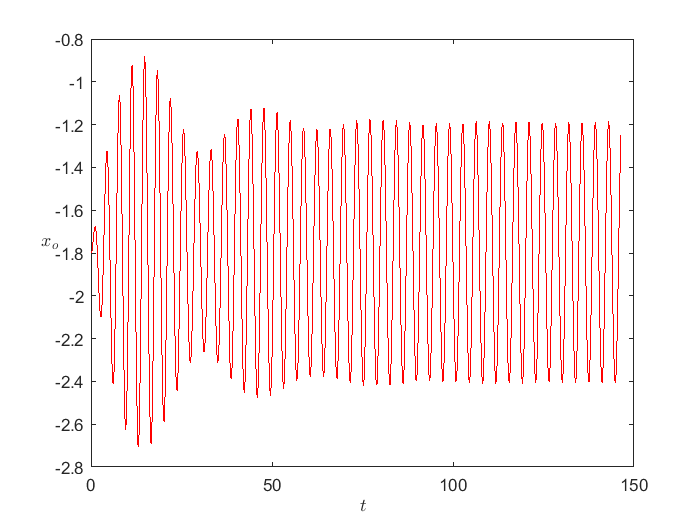
\includegraphics[width=8cm]{3_xo.png}
    \caption{振子垂荡位移-时间关系图}
  \label{zhengzi chui}
    \end{minipage}
    \begin{minipage}[t]{0.48\textwidth}
    \centering
    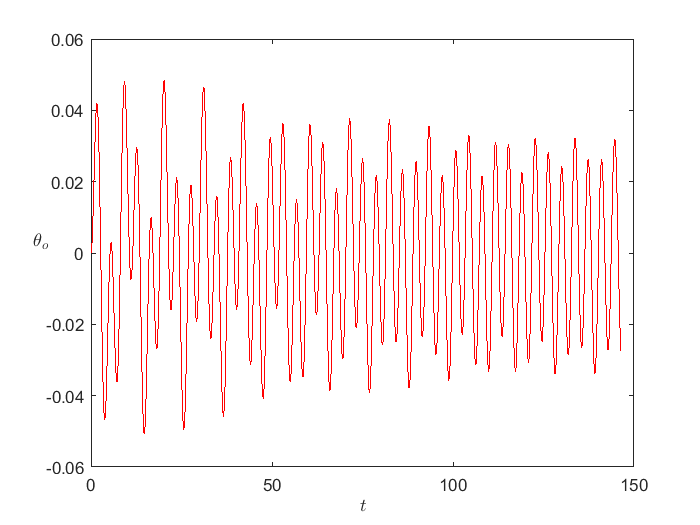
\includegraphics[width=8cm]{3_thetao.png}
    \caption{振子纵摇角位移-时间关系图}
    \label{zhengzi jiao}
    \end{minipage}
    \end{figure}

\newpage


浮子和振子在10$s$、20$s$、40$s$、60$s$、100$s$的垂荡位移与速度和纵摇角位移与角速度如表3、4所示:

% Please add the following required packages to your document preamble:
% \usepackage{multirow}
\begin{table}[!htbp]
\setlength{\belowcaptionskip}{0.2cm}
\caption{浮子的运动状态}
\centering
\begin{tabular}{|c|cccc|}
\hline
\multirow{2}{*}{\textbf{时间 (s)}} & \multicolumn{4}{c|}{\textbf{浮子}}                                                                                                               \\ \cline{2-5} 
                                 & \multicolumn{1}{c|}{\textbf{垂荡位移 (m)}} & \multicolumn{1}{c|}{\textbf{垂荡速度 (m/s)}} & \multicolumn{1}{c|}{\textbf{纵摇角位移}} & \textbf{纵摇角速度 ($\bm{s^{-1}}$)} \\ \hline
10                               & \multicolumn{1}{c|}{-2.530205404}      & \multicolumn{1}{c|}{0.969656259}         & \multicolumn{1}{c|}{0.025905358}    & -0.044915317         \\ \hline
20                               & \multicolumn{1}{c|}{-2.707149731}      & \multicolumn{1}{c|}{-0.272495862}        & \multicolumn{1}{c|}{0.04530003}     & 0.015251541          \\ \hline
40                               & \multicolumn{1}{c|}{-1.630977902}      & \multicolumn{1}{c|}{0.758080582}         & \multicolumn{1}{c|}{-0.013147645}   & -0.015661311         \\ \hline
60                               & \multicolumn{1}{c|}{-2.321632588}      & \multicolumn{1}{c|}{-0.723166485}        & \multicolumn{1}{c|}{0.024724855}    & 0.0384184            \\ \hline
100                              & \multicolumn{1}{c|}{-2.050102029}      & \multicolumn{1}{c|}{-0.94791551}         & \multicolumn{1}{c|}{0.005764356}    & 0.048632011          \\ \hline
\end{tabular}

\end{table}


% Please add the following required packages to your document preamble:
% \usepackage{multirow}
\begin{table}[!htbp]
\setlength{\belowcaptionskip}{0.2cm}
\caption{振子的运动状态}
\centering
\begin{tabular}{|c|llll|}
\hline
\multirow{2}{*}{\textbf{时间 (s)}} & \multicolumn{4}{c|}{\textbf{振子}}                                                                                                                                    \\ \cline{2-5} 
                                 & \multicolumn{1}{c|}{\textbf{垂荡位移 (m)}} & \multicolumn{1}{c|}{\textbf{垂荡速度 (m/s)}} & \multicolumn{1}{c|}{\textbf{纵摇角位移}} & \multicolumn{1}{c|}{\textbf{纵摇角速度 ($\bm{s^{-1}}$)}} \\ \hline
10                               & \multicolumn{1}{l|}{-2.39872616}       & \multicolumn{1}{l|}{1.037259095}         & \multicolumn{1}{l|}{0.026936371}    & -0.046993777                              \\ \hline
20                               & \multicolumn{1}{l|}{-2.572543584}      & \multicolumn{1}{l|}{-0.322107565}        & \multicolumn{1}{l|}{0.047224723}    & 0.015357587                               \\ \hline
40                               & \multicolumn{1}{l|}{-1.405760548}      & \multicolumn{1}{l|}{0.845603018}         & \multicolumn{1}{l|}{-0.013989323}   & -0.016586873                              \\ \hline
60                               & \multicolumn{1}{l|}{-2.140468111}      & \multicolumn{1}{l|}{-0.800596124}        & \multicolumn{1}{l|}{0.025960204}    & 0.040466308                               \\ \hline
100                              & \multicolumn{1}{l|}{-1.840587578}      & \multicolumn{1}{l|}{-1.037923424}        & \multicolumn{1}{l|}{0.0060929}      & 0.050803328                               \\ \hline
\end{tabular}

\end{table}


\subsection{问题四}

\subsubsection{模型建立}

\textbf{Step 1 优化目标}

考虑波浪能系统的垂荡和纵摇运动,输出功率为直线阻尼器和旋转阻尼器功率之和,其瞬时功率表达式为\cite{唐友刚2016筏式波浪能发电装置浮体水动力相互作用与能量俘获研究}:
\begin{equation}
    P=F_{d} v_{r} + W_{d} w_{r}\label{average Power4}
\end{equation}
其中$v_{r} $为振子相对于浮子的速度,$w_{r} $为振子相对于浮子的角速度。

由式(\ref{Q1fPTO})、(\ref{Q3fPTO})、(\ref{average Power4})可得:
\begin{equation}
    P=c_{s} v_{r}^2 + c_{t} w_{r}^2 \label{shunshigonglv4}
\end{equation}

平均输出功率为:
\begin{equation}
    \overline{P}=\frac{1}{T}\int_{0}^{T}{P}\,{\rm d}t\label{pingjungonglv4}
\end{equation}

根据问题二,需要求解设定阻尼系数下允许的PTO系统最大平均输出功率,则目标为平均输出功率最大。结合式(\ref{shunshigonglv4})、(\ref{pingjungonglv4}),优化目标为:

$$
\max \quad \overline{P}=\frac{1}{T}\int_{0}^{T}{(c_{s} v_{r}^2 + c_{t} w_{r}^2)}\,{\rm d}t
$$

\textbf{Step 2 约束条件}

根据题目信息,约束条件为阻尼系数$c_s$和$c_t$的取值范围。
        \begin{equation}
            \left\{\begin{matrix}
            0\leq c_{s}\leq 100000 \\
            0\leq c_{t}\leq 100000 \\
            
            \end{matrix}\right.
        \end{equation}
        其中,$\sigma$为比例系数,$r$为幂指数。
    

\textbf{Step 3 模型综合}

综上所述,建立最优阻尼系数的输出功率模型综合如下:

\begin{equation}
    \left\{\begin{matrix}
        \max & \overline{P}=\frac{1}{T}\int_{0}^{T}{(c_{s} v_{r}^2 + c_{t} w_{r}^2)}\,{\rm d}t\\
        s.t. & 0 \leq c_s\leq 100000 \\
            & 0 \leq c_t\leq 100000 \\
            &  m_f \ddot x_f = F_w+F_{HS}+F_a+F_d+F_{PTO}\\
            &  m_o\ddot x_o = F_{PTO}^{'}-G_o\\
            & I_{f} \ddot \theta_{f} = M_w+M_{HS}+M_a+M_{Wd}+M_{PTO}\\
            & I_{o} \ddot \theta_{o} = M_{PTO}^{'}+M_{G}
    \end{matrix}
    \right.
\end{equation}
        



\subsubsection{模型求解}
为了求解平均功率计算式中所需的$v_r$和$w_r$,需结合第三问中所建立的
浮子、振子的运动模型,将浮子、振子的运动方程与两种情况下的平均功率计算式、约束条件结合后可得最终的目标优化方程组。
\begin{equation}
    \left\{\begin{matrix}
        \max & \overline{P}=\frac{1}{T}\Sigma{(c_{s} v_{r}^2 + c_{t} w_{r}^2) \Delta t}\\
        s.t. & 0 \leq c_s\leq 100000 \\
            & 0 \leq c_t\leq 100000 \\
            &  m_f \ddot x_f = F_w+F_{HS}+F_a+F_d+F_{PTO}\\
            &  F_{PTO}^{'}-G_o=m_o\ddot x_o\\
            & I_{f} \ddot \theta_{f} = M_w+M_{HS}+M_a+M_{Wd}+M_{PTO}\\
            & I_{o} \ddot \theta_{o} = M_{PTO}^{'}+M_{G}
    \end{matrix}
    \right.
\end{equation}

  

取$\Delta t = 0.10s$,使用粒子群算法求解,得:
\begin{equation}
    \overline{P}_{max}=293.624W \quad c_s=56567.4276N\cdot s/m  \quad 56567.079N\cdot m \cdot s 
\end{equation}


%----------- 六、模型的分析与检验 ----------
%%\section{六、模型的分析与检验}

%模型的分析与检验的内容也可以放到模型的建立与求解部分,这里我们单独抽出来进行讲解,因为这部分往往是论文的加分项,很多优秀论文也会单独抽出一节来对这个内容进行讨论。

%模型的分析 :在建模比赛中模型分析主要有两种,一个是灵敏度(性)分析,另一个是误差分析。灵敏度分析是研究与分析一个系统(或模型)的状态或输出变化对系统参数或周围条件变化的敏感程度的方法。其通用的步骤是:控制其他参数不变的情况下,改变模型中某个重要参数的值,然后观察模型的结果的变化情况。误差分析是指分析模型中的误差来源,或者估算模型中存在的误差,一般用于预测问题或者数值计算类问题。

%模型的检验:模型检验可以分为两种,一种是使用模型之前应该进行的检验,例如层次分析法中一致性检验,灰色预测中的准指数规律的检验,这部分内容应该放在模型的建立部分;另一种是使用了模型后对模型的结果进行检验,数模中最常见的是稳定性检验,实际上这里的稳定性检验和前面的灵敏度分析非常类似。

\section{六、灵敏度分析}

在问题二求解最大平均输出功率中,采用了按照一定时间间隔$\Delta t$离散化处理的方法。为了探究时间间隔$\Delta t$的取值对问题答案的影响,让时间间隔$\Delta t$在当前值附近以$0.02s$的步长变化,研究问题二的结果变化程度,得到在两种情况下PTO最大平均输出功率随时间间隔$\Delta t$变化的曲线。

情况(1)阻尼系数为常量,给定阻尼系数的取值界限;

情况(2)阻尼系数为变量,与浮子和振子的相对速度的绝对值的幂成正比,给定比例系数和幂指数的取值界限。

在情况(1)的条件下TO最大平均输出功率随时间间隔$\Delta t$变化的曲线如图13;在情况(2)的条件下PTO最大平均输出功率随时间间隔$\Delta t$变化的曲线如图14。


\begin{figure}[!h]
    \centering
    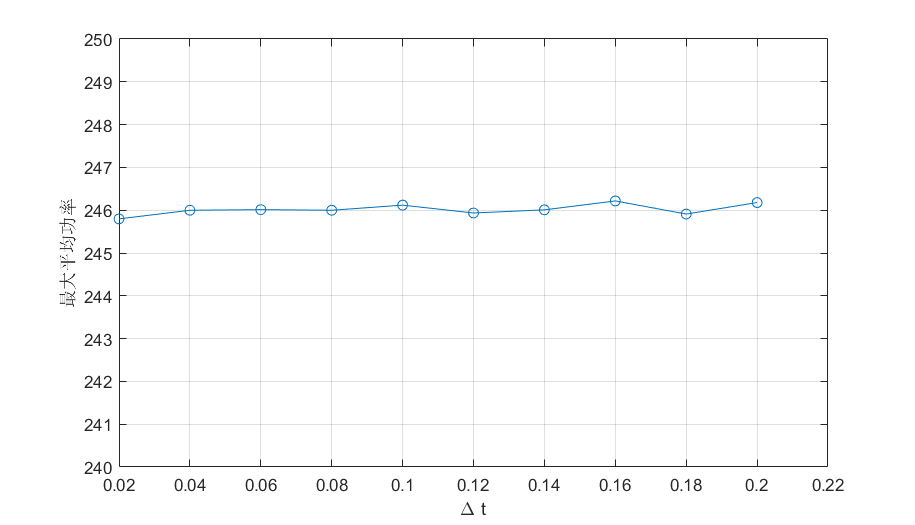
\includegraphics[width=0.5\textwidth]{灵敏度一.png}
    \caption{灵敏度分析一}
    \label{linyi}
\end{figure}

可以看出最大平均功率的变化幅度不大,此外,计算每一情况下的最优阻尼系数可知其变化范围不超过
10\%。


\begin{figure}[!h]
    \centering
    \includegraphics[width=0.5\textwidth]{untitled.png}
    \caption{灵敏度分析二}
    \label{liner}
\end{figure}

最大平均功率变化幅度亦不大,经计算,比例系数与幂指数的变化均小于10\%,综上所述
,模型较为稳定。问题四中的模型与问题二类似,其灵敏度分析过程就不在此赘述。





\section{七、模型评价与推广}

\subsection{模型的优点}
1. 在求解平均功率的大小时,通过对时间进行离散化处理,简化了平均功率的求解过程。

2. 首先单独分析波浪能转换装置的纵摇运动,再综合考虑纵摇运动与垂荡运动之间的相互影响,模型架构清晰。

3. 在问题二、四的计算结果中,浮子和振子的运动状态都趋于稳定,说明模型的可信度较高。

4. 运用了力与力矩之间的对偶性来分析浮子和振子的受力矩情况,简化了问题的求解。
% 可靠 真实 可信度 结果拟合好 通用 实用 创新  架构清晰 
\subsection{模型的缺点}

1. 在受力分析时忽略了中轴、底座、隔层及PTO的质量和各种摩擦,考虑的不够全面。

2. 计算功率时忽略了各种能的功率损耗,和真实条件有所偏差。

3. 以转轴为浮子转动的的转轴,忽略了在浮子运动过程中,转动轴的转轴的轻微变化。
\subsection{模型的改进与推广}
1. 全面考虑波浪能转换装置的受力情况。

2. 计算功率时考虑能量转换过程中的能量损耗。

3. 在浮子运动过程中,考虑浮子转动轴的变化

4. 模型中对于浮子、振子运动情况建立的模型可以用于分析其他模式下的波浪能转换装置。

%----------- 参考文献 ----------
\bibliographystyle{unsrt} %规定了参考文献的格式
\begin{center}
  %\bibitem  [序号]  {标签}  按格式给出文献名字
 %\bibitem[1]{bg}焦进莉,六西格玛方法在提升SMT回流焊过程质量中的应用研究,上海交通大学,2012年第05期
 %上面是一种简单的文献给出方式,最好卸载referenece.bib中
\bibliography{reference} %调出LaTeX生成参考文献列表
\end{center}

%----------- 附录 ----------

\newpage
\section{附录}

\noindent \large \textbf{A.支撑材料列表} \\ %换行 

\begin{itemize}
\item 问题一
\begin{itemize}
    \item t\_1.m \quad ——求解问题一程序
    \item V.m \quad ——计算体积的函数
    \item result1-1.xlsx \quad ——题目要求结果
    \item result1-2.xlsx \quad ——题目要求结果
    \item result1-1\_dis.xlsx \quad ——用于论文中展示(10s, 20s, 40s, 60s, 100s)
    \item result1-2\_dis.xlsx \quad ——用于论文中展示(10s, 20s, 40s, 60s, 100s)
    \item 附件3.xlsx
\end{itemize}
    
\item 问题二
\begin{itemize}
    \item t\_2.m \quad ——求解问题二程序
    \item V.m \quad ——计算体积的函数
    \item P.m \quad ——计算平均输出功率的函数
    \item 2.csv \quad ——问题二结果
    \item 2-1.csv \quad ——问题二灵敏度分析
    \item 2-2.csv \quad ——问题二灵敏度分析
\end{itemize}

\item 问题三
\begin{itemize}
    \item t\_3.m \quad ——求解问题三程序
    \item V.m \quad ——计算体积的函数
    \item result3.xlsx \quad ——题目要求结果
    \item result3\_dis.xlsx \quad ——用于论文中展示(10s, 20s, 40s, 60s, 100s)
    \item 附件3.xlsx
\end{itemize}

\newpage
\item 问题四
\begin{itemize}
    \item t\_4.m \quad ——求解问题四程序
    \item V.m \quad ——计算体积的函数
    \item P4.m ——计算问题四平均输出功率的函数
\end{itemize}

\item images/ \quad ——存放代码运行得到的部分图的目录
\item 论文相关材料/ \quad ——存放.tex源文件等论文相关材料的目录


\end{itemize}

\\

\noindent \large \textbf{B.源代码} \\ \\ %换行
\textbf{t\_1.m}
\begin{lstlisting}
clear, clc
a = readmatrix('附件3.xlsx');
a = a(:, 2:end);

i = 1;
w = a(i, 1);
m_a1 = a(i, 2);
c1 = a(i, 4);
f = a(i, 6);

m_f = 4866;
r = 1;
m_o = 2433;
rho = 1025;
k = 80000;
g = 9.8;
l0 = 0.5;

xf0 = -2;
xo0 = -1.8;

c = 10000;

T = 2 * pi / w;

dp_c=@(t,p,c)[p(2); 
          (-(c1 + c) * p(2) - k * p(1) + c * p(4) + k * p(3) - k * l0 + ...
          rho * g * V(p(1)) - m_f * g +...
          f * cos(w * t)) / (m_a1 + m_f);
          p(4); 
          (c * p(4) + k * p(3) - c * p(2) - k * p(1) + m_o * g - k * l0) / (-m_o);];
dp1 = @(t,p)dp_c(t, p, c);
dp2 = @(t,p)dp_c(t, p, c*(abs(p(2) - p(4))^0.5));
      
sol1=ode45(dp1,[0,40*T],[-2 0 -1.8 0]);
sol2=ode45(dp2,[0,40*T],[-2 0 -1.8 0]);


%保存结果
t = 0:0.2:40*T;
t_dis = [10, 20, 40, 60, 100];
% result1-1
p1 = deval(sol1,t);
xf1 = p1(1,:);
vf1 = p1(2,:);
xo1 = p1(3,:);
vo1 = p1(4,:);

figure;
plot(t, xf1);
xlabel('$t/s$', 'Interpreter', 'latex', 'fontsize',16)
ylabel('$x_f/m$', 'Interpreter', 'latex', 'fontsize',16)

figure;
plot(t, xo1, 'r');
xlabel('$t/s$', 'Interpreter', 'latex', 'fontsize',16)
ylabel('$x_o/m$', 'Interpreter', 'latex', 'fontsize',16)

result1 = [t; xf1; vf1; xo1; vo1]';
filename = 'result1-1.xlsx';
writematrix(result1,filename,'Sheet',1,'Range','A3:E900')

% 论文展现
p1_dis = deval(sol1,t_dis);
xf1_dis = p1_dis(1,:);
vf1_dis = p1_dis(2,:);
xo1_dis = p1_dis(3,:);
vo1_dis = p1_dis(4,:);
result1_dis = [t_dis; xf1_dis; vf1_dis; xo1_dis; vo1_dis]';
filename = 'result1-1_dis.xlsx';
writematrix(result1_dis,filename,'Sheet',1,'Range','A3:E7')

% result1-2
p2 = deval(sol2,t);
xf2 = p2(1,:);
vf2 = p2(2,:);
xo2 = p2(3,:);
vo2 = p2(4,:);

figure;
plot(t, xf2);
xlabel('$t/s$', 'Interpreter', 'latex', 'fontsize',16)
ylabel('$x_f/m$', 'Interpreter', 'latex', 'fontsize',16)

figure;
plot(t, xo2, 'r');
xlabel('$t/s$', 'Interpreter', 'latex', 'fontsize',16)
ylabel('$x_o/m$', 'Interpreter', 'latex', 'fontsize',16)

result2 = [t; xf2; vf2; xo2; vo2]';
filename = 'result1-2.xlsx';
writematrix(result2,filename,'Sheet',1,'Range','A3:E900')

% 论文展现
p2_dis = deval(sol2,t_dis);
xf2_dis = p2_dis(1,:);
vf2_dis = p2_dis(2,:);
xo2_dis = p2_dis(3,:);
vo2_dis = p2_dis(4,:);
result2_dis = [t_dis; xf2_dis; vf2_dis; xo2_dis; vo2_dis]';
filename = 'result1-2_dis.xlsx';
writematrix(result2_dis,filename,'Sheet',1,'Range','A3:E7')
\end{lstlisting}

\noindent\textbf{V.m}
\begin{lstlisting}
function v = V(xf)
    r = 1;
    v = 0;
    if xf >= 0.8
        v = 0;
    elseif xf > 0
        v = pi * (r ^ 2) * ((0.8 - xf) ^ 3) / (0.8 ^ 2) / 3;
    elseif xf > -3
        v = 0.8 * pi / 3 - pi * (r ^ 2) * xf;
    else
        v = 9.8 * pi / 3;
    end
end
\end{lstlisting}

\noindent\textbf{t\_2.m}
\begin{lstlisting}
clear, clc

delta_T = [0.2, 0.18, 0.16, 0.14, 0.12, 0.10, 0.08, 0.06, 0.04, 0.02];

for num=1:length(delta_T)
    delta_t = delta_T(num);
    '初始化种群----------------';
    %'适应度函数定义';
    %f= @(x)x .* sin(x) .* cos(2 * x) - 2 * x .* sin(3 * x); % 函数表达式(适应度函数)
    N = 100;                         % 种群个数
    %d = 1;                          % 空间维数
    d = 2;                          % 空间维数
    ger = 150;                      % 最大迭代次数
    %limit = [0, 100000];                % 设置位置参数限制  d x 2 (d维,上下限)
    limit = [0, 100000; 0, 1];                % 设置位置参数限制  d x 2 (d维,上下限)
    %vlimit = [-1, 1];               % 设置速度限制  d x 2 (d维,上下限)
    vlimit = [-1, 1; -0.01, 0.01];               % 设置速度限制  d x 2 (d维,上下限)
    w = 0.8;                        % 惯性权重
    c1 = 0.5;                       % 自我学习因子
    c2 = 0.5;
    % 群体学习因子
    for i = 1:d
        x(:,i) = limit(i, 1) + (limit(i, 2) - limit(i, 1)) * rand(N, 1);%初始种群的位置
    end
    v = rand(N, d);                  % 初始种群的速度
    xm = x;                          % 每个个体的历史最佳位置
    ym = zeros(1, d);                % 种群的历史最佳位置
    fxm = zeros(N, 1);               % 每个个体的历史最佳适应度
    fym = -inf;                      % 种群历史最佳适应度(寻max则初始化为-inf,寻min则初始化为inf)
    '-----------------------------------------------';

    '群体更新';
    record = zeros(ger, 1);          % 记录器(记录每次迭代的群体最佳适应度)
    for iter = 1:ger
        fx = zeros(N, 1);
        for i = 1:N
            %fx(i) = P(x(i), 0, delta_t); % 个体当前适应度
            fx(i) = P(x(i, 1), x(i, 2), delta_t); % 个体当前适应度
        end
        '更新个体历史最佳适应度和个体历史最佳位置';
        for i = 1:N      
            if fxm(i) < fx(i) % < / > --------------------------
                fxm(i) = fx(i);     % 更新个体历史最佳适应度
                xm(i,:) = x(i,:);   % 更新个体历史最佳位置
            end 
        end

        '更新群体历史最佳适应度和群体历史最佳位置';
        if fym < max(fxm) % < / > --------------------------------
            [fym, nmax] = max(fxm);   % 更新群体历史最佳适应度-----
            ym = xm(nmax, :);      % 更新群体历史最佳位置
        end

        '速度更新';
        v = v * w + c1 * rand * (xm - x) + c2 * rand * (repmat(ym, N, 1) - x);% 速度更新
        % 边界速度处理--------------------------------------------
        new_v = zeros(N, d);
        for i = 1:d
            vi = v(:,i);
            vi(vi > vlimit(i,2)) = vlimit(i,2);
            vi(vi < vlimit(i,1)) = vlimit(i,1);
            new_v(:,i) = vi;
        end
        v = new_v;

        '位置更新';
        x = x + v; % 位置更新
        % 边界位置处理---------------------------------
        new_x = zeros(N, d);
        for i = 1:d
            xi = x(:,i);
            xi(xi > limit(i,2)) = limit(i,2);
            xi(xi < limit(i,1)) = limit(i,1);
            new_x(:,i) = xi;
        end
        x = new_x;
        record(iter) = fym; % 最佳适应度记录
    end

    figure(3);plot(record);title('收敛过程')
    % f = fopen('2_1.csv', 'a');
    f = fopen('2_2.csv', 'a');
    fprintf(f,'delta_t:%.2f, 最大值:%.4f, 变量取值:%.4f, %.2f\n', delta_t, fym, ym(1), ym(2));
    fclose(f);
    disp(['最大值:',num2str(fym)]);
    disp(['变量取值:',num2str(ym(1)), ' ', num2str(ym(2))]);
end
\end{lstlisting}

\noindent\textbf{P.m}
\begin{lstlisting}
function ans = P(c, n, delta_t)
    w = 2.2143;
    m_a1 = 1165.992;
    c1 = 167.8395;
    f = 4890;

    m_f = 4866;
    r = 1;
    m_o = 2433;
    rho = 1025;
    k = 80000;
    g = 9.8;
    l0 = 0.5;

    xf0 = -2;
    xo0 = -1.8;

    %c = 10000;

    T = 2 * pi / w;

    dp_c=@(t,p,c)[p(2); 
              (-(c1 + c) * p(2) - k * p(1) + c * p(4) + k * p(3) - k * l0 + ...
              rho * g * V(p(1)) - m_f * g +...
              f * cos(w * t)) / (m_a1 + m_f);
              p(4); 
              (c * p(4) + k * p(3) - c * p(2) - k * p(1) + m_o * g - k * l0) / (-m_o);];
    dp1 = @(t,p)dp_c(t, p, c);
    dp2 = @(t,p)dp_c(t, p, c*((abs(p(2) - p(4)))^n));
    sol1=ode45(dp2,[0,40*T],[-2 0 -1.8 0]);
    t = 0:delta_t:40*T;
    p1 = deval(sol1,t);
    xf1 = p1(1,:);
    vf1 = p1(2,:);
    xo1 = p1(3,:);
    vo1 = p1(4,:);
    p =  c * (vo1 - vf1) .* (vo1 - vf1);
    ans = sum(p) * delta_t / (40*T);
end
\end{lstlisting}

\noindent\textbf{t\_3.m}
\begin{lstlisting}
clear, clc
a = readmatrix('附件3.xlsx');
a = a(:, 2:end);

i = 3;
w = a(i, 1);
m_a1 = a(i, 2);
Ia = a(i, 3);
c1 = a(i, 4);
cp = a(i, 5);
f = a(i, 6);
L = a(i, 7);

m_f = 4866;
Rf = 1;
Hf1 = 3;
Hf2 = 0.8;
Sf1 = pi*Rf^2;
Sf2 = pi*Rf^2;
Sf3 = 2*pi*Rf*Hf1;
l = sqrt(Hf2^2 + Rf^2);
Sf4 = pi*Rf*l;
mf1 = Sf1 / (Sf1 + Sf2 + Sf3 + Sf4) * m_f;
mf2 = Sf2 / (Sf1 + Sf2 + Sf3 + Sf4) * m_f;
mf3 = Sf3 / (Sf1 + Sf2 + Sf3 + Sf4) * m_f;
mf4 = Sf4 / (Sf1 + Sf2 + Sf3 + Sf4) * m_f;
If1 = 1 / 4 * mf1 * Rf^2 + mf1 * Hf1^2;
If2 = 1 / 4 * mf2 * Rf^2;
If3 = 1 / 2 * mf3 * Rf^2 + 1 / 12 * mf3 * Hf1^2 + mf3 * (Hf1 / 2)^2;
dh = [0.01:0.01:Hf2];
dr = dh * Rf / Hf2;
dl = 2 * pi * dr;
dm = mf4 / (sum(dl)) * dl;
If4 = 1 / 2 * dm.*(dr.^2) + dm.*((Hf2 - dh).^2);
If4 = sum(If4);

If = If1 + If2 + If3 + If4;

m_o = 2433;
Ro = 0.5;
Ho = 0.5;
rho = 1025;
ks = 80000;
g = 9.8;
l0 = 0.5;
kt = 250000;
Khs = 8890.7;

xf0 = -2;
xo0 = -1.8;

c = 10000;
ct = 1000;

T = 2 * pi / w;


dp_c=@(t,p,c)[p(2); 
              (f*cos(w*t) - c1*p(2) + (rho*g*V(p(1)) - m_f*g) * cos(p(5)) +...
              (-ks*(l0 - (p(3) - p(1))) + c * (p(4) - p(2))) * cos(p(7)-p(5))) / (m_f + m_a1);
              p(4); 
              (ks*(l0 - (p(3)-p(1))) - c * (p(4)-p(2)) - m_o*g*cos(p(7))) / m_o;
              p(6);
              (L * cos(w*t) - cp*p(6) - Khs*p(5) + kt*(p(7)-p(5)) + ct*(p(8)-p(6)) -...
              m_o*g*sin(p(7))*(Ho / 2 + p(3)-p(1))) / (If + Ia);
              p(8);
              (-kt*(p(7)-p(5)) - ct*(p(8)-p(6)) + m_o*g*sin(p(7))*(Ho / 2 + p(3)-p(1))) /...
              (1 / 12 * m_o * (3*Ro^2 + Ho^2) + m_o*(Ho/2 + p(3) - p(1))^2)];

dp1 = @(t,p)dp_c(t, p, c);

sol1=ode45(dp1,[0,40*T],[-2 0 -1.8 0 0 0 0 0]);


%保存结果
t = 0:0.2:40*T;
t_dis = [10, 20, 40, 60, 100];
% result1-1
p1 = deval(sol1,t);
xf1 = p1(1,:);
vf1 = p1(2,:);
xo1 = p1(3,:);
vo1 = p1(4,:);
theta_f1 = p1(5,:);
wf1 = p1(6,:);
theta_o1 = p1(7,:);
wo1 = p1(8,:);

figure;
plot(t, xf1);
xlabel('$t$', 'Interpreter', 'latex')
ylabel('$x_f$', 'Interpreter', 'latex', 'Rotation', 0)

figure;
plot(t, theta_f1);
xlabel('$t$', 'Interpreter', 'latex')
ylabel('$\theta_f$', 'Interpreter', 'latex', 'Rotation', 0)

figure;
plot(t, xo1, 'r');
xlabel('$t$', 'Interpreter', 'latex')
ylabel('$x_o$', 'Interpreter', 'latex', 'Rotation', 0)

figure;
plot(t, theta_o1, 'r');
xlabel('$t$', 'Interpreter', 'latex')
ylabel('$\theta_o$', 'Interpreter', 'latex', 'Rotation', 0)

result3 = [t; xf1; vf1; theta_f1; wf1; xo1; vo1; theta_o1; wo1]';
filename = 'result3.xlsx';
writematrix(result3,filename,'Sheet',1,'Range','A3:I735')

% 论文展现
p1_dis = deval(sol1,t_dis);
xf1_dis = p1_dis(1,:);
vf1_dis = p1_dis(2,:);
xo1_dis = p1_dis(3,:);
vo1_dis = p1_dis(4,:);
theta_f1_dis = p1_dis(5,:);
wf1_dis = p1_dis(6,:);
theta_o1_dis = p1_dis(7,:);
wo1_dis = p1_dis(8,:);
result3_dis = [t_dis; xf1_dis; vf1_dis; theta_f1_dis; wf1_dis; xo1_dis; vo1_dis; theta_o1_dis; wo1_dis]';
filename = 'result3_dis.xlsx';
writematrix(result3_dis,filename,'Sheet',1,'Range','A3:I7')
\end{lstlisting}

\noindent\textbf{t\_4.m}
\begin{lstlisting}
clear, clc

%delta_T = [0.14, 0.12, 0.10, 0.08, 0.06, 0.04, 0.02];
delta_T = [0.10];

for num=1:5
    %delta_t = delta_T(num);
    delta_t = delta_T(1);
    '初始化种群---------------';
    %'适应度函数定义';
    %f= @(x)x .* sin(x) .* cos(2 * x) - 2 * x .* sin(3 * x); % 函数表达式(适应度函数)
    N = 100;                         % 种群个数
    %d = 1;                          % 空间维数
    d = 2;                          % 空间维数
    ger = 100;                      % 最大迭代次数
    %limit = [0, 100000];                % 设置位置参数限制  d x 2 (d维,上下限)
    limit = [0, 100000; 0, 100000];                % 设置位置参数限制  d x 2 (d维,上下限)
    %vlimit = [-1, 1];               % 设置速度限制  d x 2 (d维,上下限)
    vlimit = [-1, 1; -1, 1];               % 设置速度限制  d x 2 (d维,上下限)
    w = 0.8;                        % 惯性权重
    c1 = 0.5;                       % 自我学习因子
    c2 = 0.5;
    % 群体学习因子
    for i = 1:d
        %x(:,i) = limit(i, 1) + (limit(i, 2) - limit(i, 1)) * rand(N, 1);%初始种群的位置
        x(:,i) = linspace(0, 100000, N)';%初始种群的位置
    end
    v = rand(N, d);                  % 初始种群的速度
    xm = x;                          % 每个个体的历史最佳位置
    ym = zeros(1, d);                % 种群的历史最佳位置
    fxm = zeros(N, 1);               % 每个个体的历史最佳适应度
    fym = -inf;                      % 种群历史最佳适应度(寻max则初始化为-inf,寻min则初始化为inf)
    '-------------------------';

    '群体更新';
    record = zeros(ger, 1);          % 记录器(记录每次迭代的群体最佳适应度)
    for iter = 1:ger
        fx = zeros(N, 1);
        for i = 1:N
            %fx(i) = P(x(i), 0, delta_t); % 个体当前适应度
            fx(i) = P4(x(i, 1), x(i, 2), delta_t); % 个体当前适应度
        end
        '更新个体历史最佳适应度和个体历史最佳位置';
        for i = 1:N      
            if fxm(i) < fx(i) % < / > -----------------
                fxm(i) = fx(i);     % 更新个体历史最佳适应度
                xm(i,:) = x(i,:);   % 更新个体历史最佳位置
            end 
        end

        '更新群体历史最佳适应度和群体历史最佳位置';
        if fym < max(fxm) % < / > ----------------------------
            [fym, nmax] = max(fxm);   % 更新群体历史最佳适应度---
            ym = xm(nmax, :);      % 更新群体历史最佳位置
        end

        '速度更新';
        v = v * w + c1 * rand * (xm - x) + c2 * rand * (repmat(ym, N, 1) - x);% 速度更新
        % 边界速度处理-----------------------------------------
        new_v = zeros(N, d);
        for i = 1:d
            vi = v(:,i);
            vi(vi > vlimit(i,2)) = vlimit(i,2);
            vi(vi < vlimit(i,1)) = vlimit(i,1);
            new_v(:,i) = vi;
        end
        v = new_v;

        '位置更新';
        x = x + v; % 位置更新
        % 边界位置处理-------------------------------------------
        new_x = zeros(N, d);
        for i = 1:d
            xi = x(:,i);
            xi(xi > limit(i,2)) = limit(i,2);
            xi(xi < limit(i,1)) = limit(i,1);
            new_x(:,i) = xi;
        end
        x = new_x;
        record(iter) = fym; % 最佳适应度记录
    end

    figure(3);plot(record);title('收敛过程')
    % f = fopen('2_1.csv', 'a');
    f = fopen('4_true.csv', 'a');
    fprintf(f,'delta_t:%.2f, 最大值:%.4f, 变量取值:%.4f, %.2f\n', delta_t, fym, ym(1), ym(2));
    fclose(f);
    disp(['最大值:',num2str(fym)]);
    disp(['变量取值:',num2str(ym(1)), ' ', num2str(ym(2))]);
end
\end{lstlisting}

\noindent\textbf{P4.m}
\begin{lstlisting}
function ans = P(c, ct, delta_t)
    w = 1.9806;
    m_a1 = 1091.099;
    Ia = 7142.493;
    c1 = 528.5018;
    cp = 1655.909;
    f = 1760;
    L = 2140;

    m_f = 4866;
    Rf = 1;
    Hf1 = 3;
    Hf2 = 0.8;
    Sf1 = pi*Rf^2;
    Sf2 = pi*Rf^2;
    Sf3 = 2*pi*Rf*Hf1;
    l = sqrt(Hf2^2 + Rf^2);
    Sf4 = pi*Rf*l;
    mf1 = Sf1 / (Sf1 + Sf2 + Sf3 + Sf4) * m_f;
    mf2 = Sf2 / (Sf1 + Sf2 + Sf3 + Sf4) * m_f;
    mf3 = Sf3 / (Sf1 + Sf2 + Sf3 + Sf4) * m_f;
    mf4 = Sf4 / (Sf1 + Sf2 + Sf3 + Sf4) * m_f;
    If1 = 1 / 4 * mf1 * Rf^2 + mf1 * Hf1^2;
    If2 = 1 / 4 * mf2 * Rf^2;
    If3 = 1 / 2 * mf3 * Rf^2 + 1 / 12 * mf3 * Hf1^2 + mf3 * (Hf1 / 2)^2;
    dh = [0.01:0.01:Hf2];
    dr = dh * Rf / Hf2;
    dl = 2 * pi * dr;
    dm = mf4 / (sum(dl)) * dl;
    If4 = 1 / 2 * dm.*(dr.^2) + dm.*((Hf2 - dh).^2);
    If4 = sum(If4);

    If = If1 + If2 + If3 + If4;

    m_o = 2433;
    Ro = 0.5;
    Ho = 0.5;
    rho = 1025;
    ks = 80000;
    g = 9.8;
    l0 = 0.5;
    kt = 250000;
    Khs = 8890.7;

    xf0 = -2;
    xo0 = -1.8;


    T = 2 * pi / w;

    dp_c=@(t,p,c)[p(2); 
              (f*cos(w*t) - c1*p(2) + (rho*g*V(p(1)) - m_f*g) * cos(p(5)) +...
              (-ks*(l0 - (p(3) - p(1))) + c * (p(4) - p(2))) * cos(p(7)-p(5))) / (m_f + m_a1);
              p(4); 
              (ks*(l0 - (p(3)-p(1))) - c * (p(4)-p(2)) - m_o*g*cos(p(7))) / m_o;
              p(6);
              (L * cos(w*t) - cp*p(6) - Khs*p(5) + kt*(p(7)-p(5)) + ct*(p(8)-p(6)) -...
              m_o*g*sin(p(7))*(Ho / 2 + p(3)-p(1))) / (If + Ia);
              p(8);
              (-kt*(p(7)-p(5)) - ct*(p(8)-p(6)) + m_o*g*sin(p(7))*(Ho / 2 + p(3)-p(1))) /...
              (1 / 12 * m_o * (3*Ro^2 + Ho^2) + m_o*(Ho/2 + p(3) - p(1))^2)];
    dp1 = @(t,p)dp_c(t, p, c);

    sol1=ode45(dp1,[0,40*T],[-2 0 -1.8 0 0 0 0 0]);
    t = 0:delta_t:40*T;
    p1 = deval(sol1,t);
    xf1 = p1(1,:);
    vf1 = p1(2,:);
    xo1 = p1(3,:);
    vo1 = p1(4,:);
    theta_f1 = p1(5,:);
    wf1 = p1(6,:);
    theta_o1 = p1(7,:);
    wo1 = p1(8,:);
    p =  c * (vo1 - vf1) .* (vo1 - vf1) + ct * (wo1 - wf1) .* (wo1 - wf1);
    ans = sum(p) * delta_t / (40*T);
end
\end{lstlisting}

\end{document}